\documentclass[14pt]{extarticle}
\usepackage{fontspec}
\usepackage[ukrainian]{babel}
\usepackage[a4paper, left=20mm, top=20mm, right=10mm, bottom=20mm]{geometry}
\usepackage{indentfirst}
\usepackage{titlesec}
\usepackage{stringstrings}
\usepackage{fancyhdr}
\usepackage{enumitem}
\usepackage{tabularx, ragged2e}
\usepackage[hidelinks]{hyperref}
\usepackage{textcase}
\usepackage{url}
\usepackage{csquotes}
\usepackage[style=numeric, sorting=none]{biblatex}
\usepackage{graphicx}
\usepackage{float}
\usepackage{caption}
\usepackage{listings}
\usepackage{rotating}
\usepackage{amssymb}
\usepackage{amsmath}
\usepackage{setspace}
\usepackage{verbatim}

\lstnewenvironment{mycode}[1][]{
  \lstset{
    basicstyle=\small\ttfamily,
    captionpos=b,
    #1
  }
}{}

\DeclareCaptionLabelFormat{dstuFigLabel}{Рисунок #2}
\DeclareCaptionLabelSeparator{abobasep}{ --- }
\captionsetup[figure]{labelformat = dstuFigLabel
                     ,labelsep    = abobasep
                     }

\addbibresource{zapiska.bib}

% TODO: make section uppercase in embedded links

% Uppercase sections in ToC
\makeatletter
\let\oldcontentsline\contentsline
\def\contentsline#1#2{%
  \expandafter\ifx\csname l@#1\endcsname\l@section
    \expandafter\@firstoftwo
  \else
    \expandafter\@secondoftwo
  \fi
  {%
    \oldcontentsline{#1}{\MakeTextUppercase{#2}}%
  }{%
    \oldcontentsline{#1}{#2}%
  }%
}
\makeatother

\hypersetup{linktoc=all}

\pagestyle{fancy}
\fancyhf{}
\fancyhead[R]{\thepage}
\renewcommand{\headrule}{}
\setlength{\headheight}{17pt}

\setmainfont{Times New Roman}
\linespread{1.5}
\setlength{\parindent}{16mm}

\titleformat{\section}
  { \filcenter % center
    \fontsize{14pt}{14pt}
    \bfseries % semi bold
    \MakeUppercase
  }
  {\thesection~}
  {0pt}
  {}
\titlespacing*{\section}{0pt}{12pt}{6pt}

\titleformat{\subsection}
  { \fontsize{14pt}{14pt}
  }
  % TODO: sentence case
  {\thesubsection~}
  {0pt}
  {}
\titlespacing*{\subsection}{0pt}{6pt}{0pt}

\titleformat{\subsubsection}
  { \fontsize{14pt}{14pt}
  }
  % TODO: sentence case
  {\thesubsubsection~}
  {0pt}
  {}
\titlespacing*{\subsubsection}{0pt}{6pt}{0pt}

% all sections will start at new page
\let\oldsection\section
\renewcommand{\section}{\clearpage\oldsection}

\newcommand{\unnumberedSection}[1]{%
  \section*{#1}%
  \phantomsection
  \addcontentsline{toc}{section}{#1}%
}

\newcommand{\unnumberedSubsection}[1]{%
  \subsection*{#1}%
  \addcontentsline{toc}{subsection}{#1}%
}

\begin{document}

\begin{spacing}{1}
\begin{center}
  Міністерство освіти і науки України\\
  Український державний університет науки і технологій\\

  \vspace{\baselineskip}

  Факультет «Комп'ютерні технології і системи»\\
  Кафедра «Комп'ютерні інформаційні технології»\\

  \vspace{\baselineskip}
  \vspace{\baselineskip}

  {\fontsize{18}{18}\selectfont  Пояснювальна записка}\\
  до кваліфікаційної роботи бакалавра
\end{center}
на тему: «Розробка засобів підбору та перевірки коректності
УДК-шифрів наукових робіт»\\
за освітньою програмою: «Інженерія програмного забезпечення»\\
зі  спеціальності: «121 Інженерія програмного забезпечення»\\
Виконав: студент групи «ПЗ1911»\\

\noindent
\begin{tabularx}{\textwidth}{@{}>{\RaggedRight}lXp{0.7cm}l}
                  &                                             & & /Данило САФОНОВ/ \\ \cline{2-2} \cline{4-4}
                  & \fontsize{9}{9}\selectfont(підпис студента) & & \fontsize{9}{9}\selectfont(Ім’я ПРІЗВИЩЕ) \\
  Керівник:       &                                             & & /доц. Олена КУРОП'ЯТНИК/ \\ \cline{2-2} \cline{4-4}
                  & \fontsize{9}{9}\selectfont(підпис)          & & \fontsize{9}{9}\selectfont(посада, Ім’я ПРІЗВИЩЕ) \\
  Нормоконтролер: &                                             & & /доц. Світлана ВОЛКОВА/ \\ \cline{2-2} \cline{4-4}
                  & \fontsize{9}{9}\selectfont(підпис)          & & \fontsize{9}{9}\selectfont(посада, Ім’я ПРІЗВИЩЕ) \\
\end{tabularx}

\vspace{\baselineskip}
\vspace{\baselineskip}
\vspace{\baselineskip}
\vspace{\baselineskip}
\vspace{\baselineskip}
\vspace{\baselineskip}

\begin{flushright}
  \begin{tabular}{ll}
    \multicolumn{2}{l}{Засвідчую, що у цій роботі немає запозичень з}\\
    \multicolumn{2}{l}{праць інших авторів без відповідних посилань.}\\
    Студент & \\ \cline{2-2}
            & \fontsize{10}{10}\selectfont(підпис) \\
  \end{tabular}
\end{flushright}

\vspace*{\fill}
\centerline{Дніпро – 2023 рік}
\end{spacing}

\thispagestyle{empty}

\newpage

\begin{spacing}{1}
\begin{center}
  Ministry of Education and Science of Ukraine \\
  Ukrainian State University of Science and Technologies

  \vspace{\baselineskip}

  Faculty «Computer technologies and systems»\\
  Department «Computer information technology»\\

  \vspace{\baselineskip}

  {\fontsize{18}{18}\selectfont Explanatory Note}\\
  to Bachelor's Thesis\\

  \vspace{\baselineskip}
\end{center}
on the topic: «Development of tools for selection and
verification of UDC codes of scientific works»\\
according to educational curriculum «Software engineering»\\
in the Speciality: «121 Software engineering»\\
\end{spacing}

\noindent
\begin{tabularx}{\textwidth}{@{}>{\RaggedRight}p{0.57\textwidth}X}
  Done by the student of the group PZ1911: & /Danylo SAFONOV/ \\ \cline{2-2}
  Scientific Supervisor:                   & /Olena KUROPIATNYK/ \\ \cline{2-2}
  Normative controller:                    & /Svitlana VOLKOVA/ \\ \cline{2-2}
\end{tabularx}

\vspace*{\fill}
\centerline{Dnipro – 2023}

\newpage

\begin{center}
  Міністерство освіти і науки України\\
  Український державний університет науки і технологій\\  
\end{center}
Факультет: Факультет «Комп'ютерні технології і системи»\\
Кафедра: «Комп'ютерні інформаційні технології»\\
Рівень вищої освіти: бакалавр\\
Освітня програма: «Інженерія програмного забезпечення»\\
Спеціальність: «121 Інженерія програмного забезпечення»

\begin{flushright}
  \begin{tabular}{@{}>{\RaggedRight}ll}
    \multicolumn{2}{r}{ЗАТВЕРДЖУЮ}\\
    \multicolumn{2}{@{}>{\RaggedRight}l}{Завідувач кафедри КІТ}\\
             & /Вадим ГОРЯЧКІН/\\ \cline{1-1}
    (підпис) & \\
    \multicolumn{2}{@{}>{\RaggedRight}l}{Дата \rule[-2pt]{0.2\linewidth}{0.4pt}}
  \end{tabular}
\end{flushright}

\centerline{\textbf{ЗАВДАННЯ}}

\noindent
на кваліфікаційну роботу бакалавра\\
студенту Сафонову Данилу Євгеновичу\\
1. Тема роботи: «Розробка засобів підбору та перевірки коректності
УДК-шифрів наукових робіт»\\
Керівник роботи: Куроп'ятник Олена Сергіївна, доцент\\
затверджена наказом № 1209 ст від 07.12.2022

\noindent
2. Строк подання студентом роботи:
xx.06.2023 р.

\noindent
3. Вихідні дані до роботи:

\noindent
4. Зміст пояснювальної записки (перелік питань, які потрібно опрацювати):\\
TODO:

\noindent
5. Перелік графічного матеріалу (з точним зазначенням обов’язкових креслень):\\
Презентація\\
Відео роботи програми\\

\newpage
\centerline{КАЛЕНДАРНИЙ ПЛАН}
\vspace{\baselineskip}

\noindent
\begin{tabularx}{\linewidth}{|c|X|c|}
  \hline
  Стадія & Зміст & Строки виконання \\
  \hline
  TODO:  & TODO: & TODO: \\
  \hline
\end{tabularx}

\vspace{\baselineskip}
\begin{flushright}
\begin{tabular}{clp{0.7cm}l}
  Студент         &                                      & & Данило САФОНОВ \\ \cline{2-2} \cline{4-4}
                  & \fontsize{10}{10}\selectfont(підпис) & & \fontsize{10}{10}\selectfont(Ім’я ПРІЗВИЩЕ) \\
  Керівник роботи &                                      & & доц. Олена КУРОП'ЯТНИК \\ \cline{2-2} \cline{4-4}
                  & \fontsize{10}{10}\selectfont(підпис) & & \fontsize{10}{10}\selectfont(посада, Ім’я ПРІЗВИЩЕ)\\
\end{tabular}
\end{flushright}

\section*{реферат}
Пояснювальна записка до кваліфікаційної роботи бакалавра:
55с., 9 рис., 3 табл., 2 додатки, 96 джерел.

Об’єкт розробки --- додаток для автоматизації підбору
та перевірки коректності УДК-шифрів наукових робіт.

Мета роботи --- розробка додатку для автоматизації підбору
та перевірки коректності УДК-шифрів наукових робіт.

Методи дослідження --- порівняльний аналіз?.

Отримані результати --- розроблений додаток?.

Значення роботи --- розроблений додаток може
бути використаний за основу для подальшої розробки.

Пояснювальна записка складається з 9 розділів:
\begin{itemize}[labelindent=\dimexpr\parindent*2\relax, leftmargin=*]
  \item перелік умовних познак, символів, скорочень і термінів ---
    структуроване перерахування, який містить в собі набір умовних познак,
    символів, скорочень та термінів, використаних у роботі, з метою уточнення,
    стандартизації та полегшення сприйняття інформації. Складаєтся з 1 сторінки;
  \item вступ --- опис суті дослідження, її значення та актуальності.
    Складаєтся з 1 сторінки;
  \item збір та аналіз вимог --- в цьому розділі приведені аналоги,
    описані можливі сценарії використання додатку,
    функціонал розподілено за сценаріями. Складаєтся з 5 сторінок;
  \item проєктування --- цей розділ деталізує архітектуру проєкту
    для полегшення подальшої розробки та підтримки додатку.
    Складаєтся з 13 сторінок; 
  \item розробка програми --- у цьому розділи описаний процес розробки програми,
    вибір алгоритмів. Також,
    розглянуті алгоритми та структура вибраних засобів програмування.
    Складаєтся з 12 сторінок;
  \item тестування та налагодження ---
    у цьому розділі розглянута проблема поширення додатку,
    порівняні різні рішення та на основі порівняння обраний найкращій підхід.
    Складаєтся з 6 сторінок;
  \item загальні висновки та рекомендації ---
    цей розділ є підсумком роботи.
    Також, наведені ідеї щодо подальшого розвитку програми.
    Складаєтся з 2 сторінок;
  \item список використаної літератури ---
    бібліографічний список використаних джерел. Складаєтся з 8 сторінок;
  \item додатки ---
    технічне завдання? та вихідний код програми. Складаєтся з 7 сторінок.
\end{itemize}

Кількість таблиць: 2шт.

Кількість рисунків: 9шт.

Ключові слова: python, spaCy, машинне навчання, обробка природної мови,
УДК, інтерфейс командного рядка, ітераційна розробка, автоматизація.

% зміст
\tableofcontents

\unnumberedSection{ПЕРЕЛІК УМОВНИХ ПОЗНАК, СИМВОЛІВ, СКОРОЧЕНЬ І ТЕРМІНІВ}
УДК --- універсальна десяткова класифікація

НР --- наукова робота

ПЗ --- програмне забезпечення

UML --- Unified Modeling Language, уніфікована мова моделювання

% ommited because it's only used for groupping
% основну частину:
  \unnumberedSection{ВСТУП}  
  Задача, яку розглядає дана робота ---
  переклад та перевірка точності перекладу текстів \cite{wiki_nlp} (НР)
  з природної мови на формальну (шифр УДК).
  
  Точність УДК шифрів є ключовою для ефективної класифікації
  та пошуку наукової літератури.
  Однак, ручний вибір та перевірка УДК шифрів вимагає значних зусиль,
  займає багато часу та супроводжується високим ризиком виникнення помилок.
  Зовнішня перевірка може зменшити ризик помилок, але вимагає додаткових зусиль.
  Натомість, автоматизоване рішення може значно зменшити час та ресурси,
  необхідні для вибору та перевірки, а також мінімізувати ризик помилок.
  Тому ця робота має на меті розробити надійний
  та ефективний автоматизований інструмент для вибору
  та перевірки УДК шифрів НР.

  % ommited because it's only used for groupping
  % основний текст кваліфікаційного проєкту (роботи):

  \section{ЗБІР ТА АНАЛІЗ ВИМОГ}

  \subsection{Універсальна десяткова класифікація}
  Універсальна десяткова класифікація (УДК) \cite{udc_wiki} —--
  бібліографічна та бібліотечна класифікація,
  представляє систематичне впорядкування всіх галузей людських знань,
  організованих як узгоджена система,
  у якій галузі знань заємопов’язані.
  
  В УДК використовуються арабські цифри в десятковому порядку.
  Кожне число розглядається як десятковий дріб
  з опущеною початковою десятковою крапкою, яка визначає порядок запису.
  Для зручності читання УДК зазвичай ставиться розділовий знак
  після кожної третьої цифри.

  Основні таблиці \cite{udc_structure_and_tables} містять різні дисципліни та галузі знань,
  розташовані в 9 основних класах, пронумерованих від 0 до 9
  (при цьому 4 клас є вільним).
  На початку кожного класу також є серія спеціальних допоміжних слів,
  які виражають аспекти, що повторюються в цьому конкретному класі.
  Основні таблиці в УДК містять понад 60 000 підрозділів.
  \begin{enumerate}
      [labelindent=\dimexpr\parindent*2\relax, leftmargin=*, start=0]
    \item Наука і знання.
    Організація.
    Комп'ютерна наука.
    Інформатика.
    Документація.
    Бібліотечна справа.
    Заклади.
    Публікації
    \item Філософія. Психологія
    \item Релігія. Теологія
    \item Суспільствознавство
    \item -
    \item Математика. Природничі науки
    \item Прикладні науки. Медицина, Техніка
    \item Мистецтво. Розваги. Спорт
    \item Мовознавство. Література
    \item Географія. Історія
  \end{enumerate}

  Загальні допоміжні засоби — концепції,
  які можна використовувати в поєднанні
  з будь-яким іншим кодом УДК з основних класів
  або з іншими загальними допоміжними засобами.
  Вони мають унікальні позначення, що виділяють їх у складних виразах.
  Звичайні допоміжні числа завжди починаються з певного символу,
  напр. = (знак рівності) завжди вводить поняття,
  що представляють мову документа;
  (0...) цифри в круглих дужках, починаючи з нуля,
  завжди представляють поняття, що позначає форму документа.
  Таким чином (075) підручник і =111 англійська мова може бути об’єднана,
  щоб виразити, наприклад, (075)=111 підручники англійською мовою,
  і в поєднанні з числами з основних таблиць
  УДК їх можна використовувати таким чином:
  2(075)=111 підручники з релігії англійською мовою,
  51(075)=111 Підручники з математики англійською мовою та ін.

  \begin{tabularx}{\dimexpr\linewidth - \parindent\relax}{cX}
    =... & Загальні допоміжні засоби мови. \\
    (0...) & Загальні допоміжні форми форми. \\
    (1/9) & Загальні допоміжні слова місця. \\
    (=...) & Загальні допоміжні ознаки людського походження,
    етнічної групи та національності. \\
    "..." & Загальні допоміжні слова часу,
    допомагає зробити хвилинний поділ часу, наприклад: "1993-1996" \\
    -0... & Загальні допоміжні характеристики загальних характеристик:
    Властивості, Матеріали, Відносини/Процеси та Особи. \\
    -02 & Загальні допоміжні властивості. \\
    -03 & Загальні допоміжні матеріали. \\
    -04 & Загальні допоміжні елементи відносин, процесів і операцій. \\
    -05 & Загальні допоміжні особи та особисті характеристики. \\
  \end{tabularx}

  Доступно кілька сполучних символів для зв’язку та розширення номерів УДК:

  \begin{tabular}{|l|l|}
    \hline
    Символ & Значення \\
    + & узгодження, доповнення \\
    / & послідовне розширення \\
    : & відношення \\
    $[~~]$ & підгрупування \\
    $*$ & Впроваджує нотацію, відмінну від УДК \\
    A/Z & Пряма алфавітна специфікація \\
    \hline
  \end{tabular}

  \subsection{Огляд аналогів}
  Широкодоступних аналогів, які б повністю відтворювали функціонал ---
  підбір кодів (або в нашому випадку класів) УДК та їх порівняння/перевірка,
  не знайдено. Під широким доступом маются на увазі комерційні
  або відкриті/безкоштовні рішення.

  Втім, існують наукові роботи із схожою метою:
  \begin{itemize}[labelindent=\dimexpr\parindent*2\relax, leftmargin=*]
    \item "Automatic classification of older electronic texts into the UDC"
      \cite{kragelj_automatic_udc_classification}
      --- ця робота ставить своєю метою розробити модель для
      класифікації старих оцифрованих текстів.
    
    \item "Service for assigning a UDC code
	    to mathematical articles based on semantic technologies"
      \cite{almukhametov_udc_code_for_math_articles} --- 
      дана робота намагаєтся вирішити проблему класифікації математичних статей.
    
    \item "A Hybrid Approach to Recommending
      Universal Decimal Classification Codes
      for Cataloguing in Slovenian Digital Libraries"
      \cite{borovic_hybrid_udc_recommendation} ---
      ця робота має на меті додаток,
      який буде пропонувати бібліотекарям УДК шифри,
      тим самим значно спрощуючи їх роботу.

    \item "Automated Subject Identification using the
      Universal Decimal Classification: The ANN Approach"
      \cite{roy_ann_approach} ---
      мета цієї роботи така ж сама що й в попереднього прикладу.

    \item "Porter advanced method for the Universal Decimal Classification"
      \cite{tretyakov_porter} --- 
      в процесі цієї роботи розроблются додаток,
      який буде пропонувати бібліотекарям УДК шифри,
      тим самим значно спрощуючи їх роботу.

  \end{itemize}

  \subsection{Аналіз проблеми та постановка задачі}
  Мета роботи ---
  розробити ПЗ для підбору та перевірки коректності УДК шифрів НР.
  Під підбором розуміється наступний функціонал --- на вході маємо текст роботи,
  на виході --- список класів та підкласів УДК (далі --- класів),
  до яких ця робота належить.
  Перевірка --- на вході маємо текст роботи та шифр,
  на виході --- згенерований шифр та оцінку схожості наданого
  та згенерованого шифрів, яким саме чином ця оцінка буде отримана,
  та як вона буде виглядати розглянемо в наступних розділах.
  
  Програму можна узагальнити до такої специфікації ---
  на вході маємо текст роботи та опціонально шифр,
  на виході маємо список класів та, якщо був наданий шифр,
  порівняльну оцінку зі згенерованими класами.

  Через те що наукові роботи можуть бути доступні у різноманітних форматах,
  варто уточнити що ПЗ буде приймати їх
  у форматі plain-text на англійській мові.

  Це можна розглядати як проблему класифікації
  \cite{multiclass_classification_wiki, statistical_classification_wiki}
  --- маємо множину об'єктів,
  які певним чином розподілені на класи (підмножини).
  Задача класифікації ---
  різновид машинного навчання
  \cite{machine_learning_wiki} (англ. machine learning, далі —-- ML).
  Розрізняють два типи навчання:
  \begin{itemize}[labelindent=\dimexpr\parindent*2\relax, leftmargin=*]
    \item навчання з учителем (англ. supervised learning) ---
    комп'ютеру надається набір даних (data set),
    в якому даним вже надано бажаний результат ---
    саме за ним комп'ютер і буде навчатись.

    \item навчання без учителя (англ. unsupervised learning) ---
    набір даних, наданий комп'ютеру, ніяк не помічається ---
    комп'ютер сам має розбити дані на деякі групи (clustering).
  \end{itemize}

  Класи заздалегідь відомі, тож навчання без учителя, в нашому випадку,
  не підходить. Крім того можна використати існуючи класифіковані роботи,
  як набір даних для навчання.
  Але отримання достатнього набору даних вимагає великих зусиль ---
  потрібно отримати декілька робіт для кожного класу та підкласу
  та їх різних комбінацій. Тож пропонується простіший алгоритм:
  \begin{enumerate}[labelindent=\dimexpr\parindent*2\relax, leftmargin=*]
    \item Витягнемо з тексту роботи ключові слова. \cite{keyword_extraction_wiki}
    \item Порівняемо ключові слова із термінами та поняттями у каталозі УДК.
  \end{enumerate}

  Останній крок є дещо проблематичним
  через те що доступ до офіційного каталогу здійснюється на платній основі ---
  такий варіант не підходить для даного випадку через відсутність фінансування.
  Але існують безкоштовні та/або відкриті каталоги
  \cite{udc_summary, udc_summary_linked},
  які можна використати замість платної версії.
  Авжеж вони мають свої недоліки, наприклад: менша частота оновлень,
  менший корпус інформації, тощо.
  Не дивлячись на ці недоліки
  вони є достатнім ресурсом для початкової версії ПЗ.
  Також за бажанням ПЗ може бути відредагованим
  у майбутньому щоб використовувати платну версію.

  \subsection{Висновки}

  Була розглянута система УДК - задача,
  яку ця робота намагаєтся вирішити/спростити,
  є трудомісткою та займає час.
  Через це доцільне створення інструмента,
  який буде хоча б частково автоматизувати цю задачу.

  Широкодоступних аналогів не знайдено,
  наукові роботи із схожою метою в більшості розглядают лише часткові рішення
  --- вони орієнтуются на деяку підмножину НР.

  \section{ПРОЄКТУВАННЯ}
  \subsection{Зовнішнє проєктування}

  Розробнику потрібна можливість тренувати модель.
  Користувачу --- отримувати припущення від натренованої моделі припущень,
  та опціонально порівнювати це припущення із припущенням користувача.
  \begin{enumerate}[labelindent=\dimexpr\parindent*2\relax, leftmargin=*]
    \item Тренування моделі припущень:
      \begin{itemize}[labelindent=\dimexpr\parindent\relax, leftmargin=*]
        \item вхід:
          \begin{itemize}[labelindent=\dimexpr\parindent\relax, leftmargin=*]
            \item модель припущень,
            \item текст;
          \end{itemize}
        \item вихід --- нова модель припущень.
      \end{itemize}
    \item Отримання припущень від моделі:
      \begin{itemize}[labelindent=\dimexpr\parindent\relax, leftmargin=*]
        \item вхід:
          \begin{itemize}[labelindent=\dimexpr\parindent\relax, leftmargin=*]
            \item модель припущень,
            \item текст;
          \end{itemize}
        \item вихід --- список класів.
      \end{itemize}
    \item Отримання припущень від моделі та порівняння із наданим шифром УДК:
      \begin{itemize}[labelindent=\dimexpr\parindent\relax, leftmargin=*]
        \item вхід:
          \begin{itemize}[labelindent=\dimexpr\parindent\relax, leftmargin=*]
            \item модель припущень,
            \item текст,
            \item список класів УДК;
          \end{itemize}
        \item вихід:
          \begin{itemize}[labelindent=\dimexpr\parindent\relax, leftmargin=*]
            \item список класів,
            \item ступінь відповідності класів.
          \end{itemize}
      \end{itemize}
  \end{enumerate}

  Розглянуті сценарії можна формалізувати у наступній use-case діаграмі
  (рис. \ref{fig:use-case}).

  \begin{figure}[H]
    \centering
    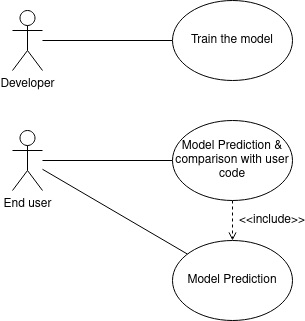
\includegraphics{use-case.drawio.png}    
    \caption{Діаграма прецедентів}
    \label{fig:use-case}
  \end{figure}

  \subsection{Внутрішнє проєктування}
  В додатку можна виділити наступні основні частини:
  \begin{itemize}[labelindent=\dimexpr\parindent*2\relax, leftmargin=*]
    \item інтерфейс користувача --- цей модуль буде перетворювати вхідні дані користувача на внутрішнє представлення та перевіряти коректність наданих даних. Також цей модуль відповідає за надання результату користувачу
    \item бекенд
      \begin{itemize}[labelindent=\dimexpr\parindent\relax, leftmargin=*]
        \item тренування моделі --- цей модуль буде додавати нові ключові слова до класів, знайдених у наданому тексті
        \item отримання припущення від моделі --- цей модуль буде надавати можливі класи до наданого тексту
        \item порівняння списків класів УДК --- цей модуль буде порівнювати два списки класів УДК, та надавати ступінь їх відповідності
      \end{itemize}
  \end{itemize}
  
  Також можна виділити такі типи даних (замість передавання рядка або числа між внутрішніми процедурами, зручніше передавати спеціалізовану структуру):
  \begin{itemize}[labelindent=\dimexpr\parindent*2\relax, leftmargin=*]
    \item наукова робота/текст,
    \item клас УДК.
  \end{itemize}

  \subsection{Проєктування архітектури системи}
  Програму розроблено ітераціями. На кожну з ітерацій виділено окрему секцію. Є два типи ітерацій:
  \begin{enumerate}[labelindent=\dimexpr\parindent*2\relax, leftmargin=*]
    \item Реалізація нового функціоналу,
    \item Вдосконалення старого функціоналу.
  \end{enumerate}
  Для простоти тестування було вирішено почати розробку з інтерфейсу користувача.
  З попередніх секцій знаємо що це буде інтерфейс командного рядка
  (CLI - Command Line Interface).

  Найпростішим варіантом
  є перевірка аргументів командного рядка у функції main,
  і після цього виклик із цими аргументами внутрішньої реалізації.

  UML-діаграма для такої моделі виглядає наступним чином
  (рис. \ref{fig:io_uml1}).
  Кінцева реалізація буде мати складнішу ієрархію модулів,
  але ця секція фокусуєтся на розробці користувацького інтерфейсу,
  тому на цьому етапі реалізація представлена як дуже простий клас.

  \begin{figure}[H]
    \centering
    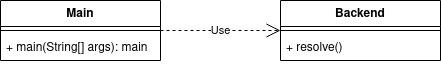
\includegraphics{io_uml1.drawio.png}    
    \caption{Діаграма високорівневого розподілення обов'язків}
    \label{fig:io_uml1}
  \end{figure}

  Алє таке рішення не є оптимальним ---
  заради простоти початкової реалізації
  втрачаєтся легкість подальшої заміні інтерфейсу.
  Тому доцільно виділити модуль який буде відповідати
  за взаємодію з користувачем.
  В нашому випадку це буде зчитування аргументів командного рядку,
  але за потреби він може бути замінений на графічний або веб-інтерфейс, тощо.
  Тепер діаграма виглядає так (рис. \ref{fig:io_uml2}).

  \begin{figure}[H]
    \centering
    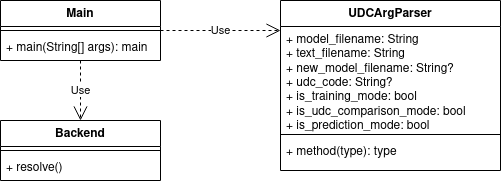
\includegraphics{io_uml2.drawio.png}    
    \caption{Виділення модуля,
    який відповідає за розпізнавання аргументів командного рядка}
    \label{fig:io_uml2}
  \end{figure}

  Тепер перед тим як викликати внутрішню реалізацію,
  main викликає клас UDCArgParser,
  який у свою чергу опрацьовує аргументи командного рядку.
  
  Хоча ця реалізація вирішує проблему відповідальності, вона додає декілька нових:
  \begin{itemize}[labelindent=\dimexpr\parindent*2\relax, leftmargin=*]
    \item по-перше, UDCArgParser зчитує аргументи комадного рядка
    у конструкторі із глобальних змінних,
    це порушує принцип Dependency Inversion \cite{DI_wiki, SOLID_wiki};
    \item по-друге, змінні is\_training\_mode, is\_udc\_comparison\_mode та \\ is\_prediction\_mode є взаємовиключними.
  \end{itemize}

  Для вирішення другої проблеми, потрібно скористатися поліморфізмом
  \cite{Polymorphism_wiki, Subtyping_wiki, Dynamic_dispatch_wiki}
  і замінити ці три змінні на одну,
  яка буде приймати значення одного з трьох підкласів.
  Іншими словами, треба заміни три взаємовиключні булеві змінні
  на одну змінну типу перечислення.
  З цими змінами UML-діаграма виглядає наступним чином (рис. \ref{fig:io_uml3}).

  \begin{figure}[H]
    \centering
    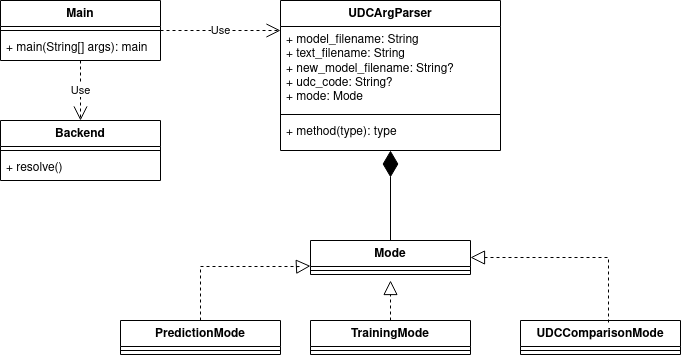
\includegraphics[width=\textwidth]{io_uml3.drawio.png}    
    \caption{Виділення типів,
    які відповідають за внутрішне представлення режиму роботи програми}
    \label{fig:io_uml3}
  \end{figure}
  
  Тепер клас Mode та його підкласи відповідають за представлення режиму,
  алє клас UDCArgParser має змінні new\_model\_filename та udc\_code,
  які в залежності від значення Mode завжди будуть NULL,
  тому доцільно перенести усі значення до підкласів Mode,
  перетворюючи тим самим це перечислення на алгебраічний тип данних
  \cite{ADT_wiki}.
  
  Доцільно помітити що алгебраічні типи даних відсутні в ООП та мові Python,
  тому вони будуть ємульовані з допомогою наслідування
  \cite{Code_complete_34_4, ADT_composition_over_inheritance}.
  
  Таким чином UDCArgParser дійсно буде мати тільки одну відповідальність ---
  перетворення аргументів командного рядка на об'єкт Mode.
  А Mode у свою чергу відповідає за представлення даних,
  які будуть надані внутрішній реалізації.
  Після цих змін UML-діаграма буде виглядати так (рис. \ref{fig:io_uml4}).

  \begin{figure}[H]
    \centering
    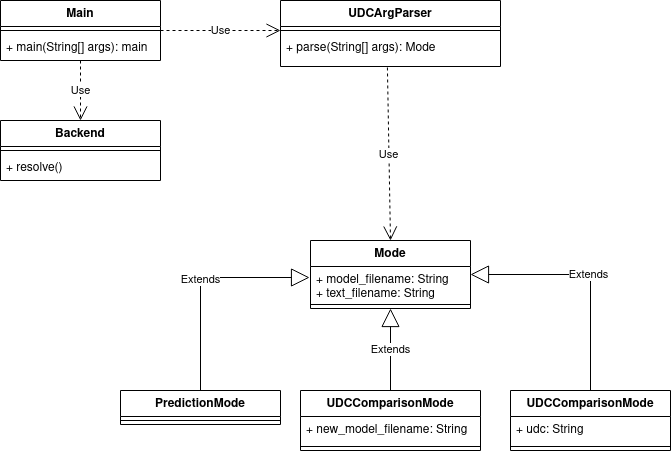
\includegraphics[width=\textwidth]{io_uml4.drawio.png}    
    \caption{Перенесення атрибутів режиму роботи до відповідних типів}
    \label{fig:io_uml4}
  \end{figure}
  
  Нова версія набагато краще попередніх, особливо першої.
  Втім, не усі недоліки були всунуті.
  
  Тип Mode містить поля model\_filename та text\_filename
  --- вони будуть передані в Backend
  (це не показано на діаграмах, тому теж є недоліком).
  Внутрішній реалізації потрібен вміст цих файлів,
  насправді внутрішня реалізація навіть не повинна знати що це вміст файлів,
  а не, наприклад, вміст текстового поля у графічному інтерфейсі, тощо.
  Тому доцільно:
    \begin{enumerate}[labelindent=\dimexpr\parindent\relax, leftmargin=*]
      \item Прибрати слово filename з обох полів,
      \item Виділити типи для цих значень ---
      таким чином ми зможемо робити майбутні зміни лише в одному місці
      \cite{Code_complete_5_3}
    \end{enumerate}
    
  Також присутня змінна new\_model\_filename в UDCComparisonMode ---
  вона так само не є важливою дла внутрішньої реалізації,
  а тільки для інтерфейсу користувача.
  Через те що для внутрішньої реалізації це буде одним з результатів
  (також можуть бути припущення щодо класів УДК та точності припущення,
  зробленного користувачем),
  це потрібно формалізувати в інтерфейсі класу Backend.
  
  Крім того, з попереднього пункту видно
  що потрібно формалізувати тип результату виконання внутрішньої реалізації.
  Втім, через те що маєтся чітка відовідність між підкласами Mode
  та типом (типами) результата внутрішньої реалізації доцільно розділити
  ці дії (режими роботи додатку) на окремі методи в класах Main та Backend.

  У новій діаграмі (рис. \ref{fig:io_uml5})
  виділено типи UdcPredictorModel та UdcPredictorInput-Text,
  також явно показано залежність внутрішньої реалізації від типу Mode.

  UDCArgParser тепер має відповідальність
  за зчитування файлів за наданими іменами,
  але саме зчитування оброблюєтся внутрішньою бібліотекою мови Python,
  тому це не є порушення принципу єдиної відповідальності \cite{SRP_wiki}.
  Ця залежність не показана на діаграмі тому що вона подразумеваєтся/implied
  (я не знаю как перевести єто слово, googletranslate предлагает вообще не то)
  як атомарний функціонал мови, як і багато інших дещо простіших речей.

  Для вирішення інших проблем, описаних в попередній ітерації,
  краще розпочати з конкретизації внутрішньої реалізації.
  Через те що кожному з вхідних підтипів Mode буде відповідати новий формат
  результату, доцільно розділити метод resolve, на три різні.
  Крім того, ми можемо позбавитися залежності між
  внутрішньою реалізацією та типом Mode ---
  методи можуть приймати декілька параметрів,
  щодо результатів, функції в мові Python (та інших сучасних)
  можна повертати декілька значень
  \cite{python3_tuples_and_sequences}.

  \begin{sidewaysfigure}[htbp]
    \centering
    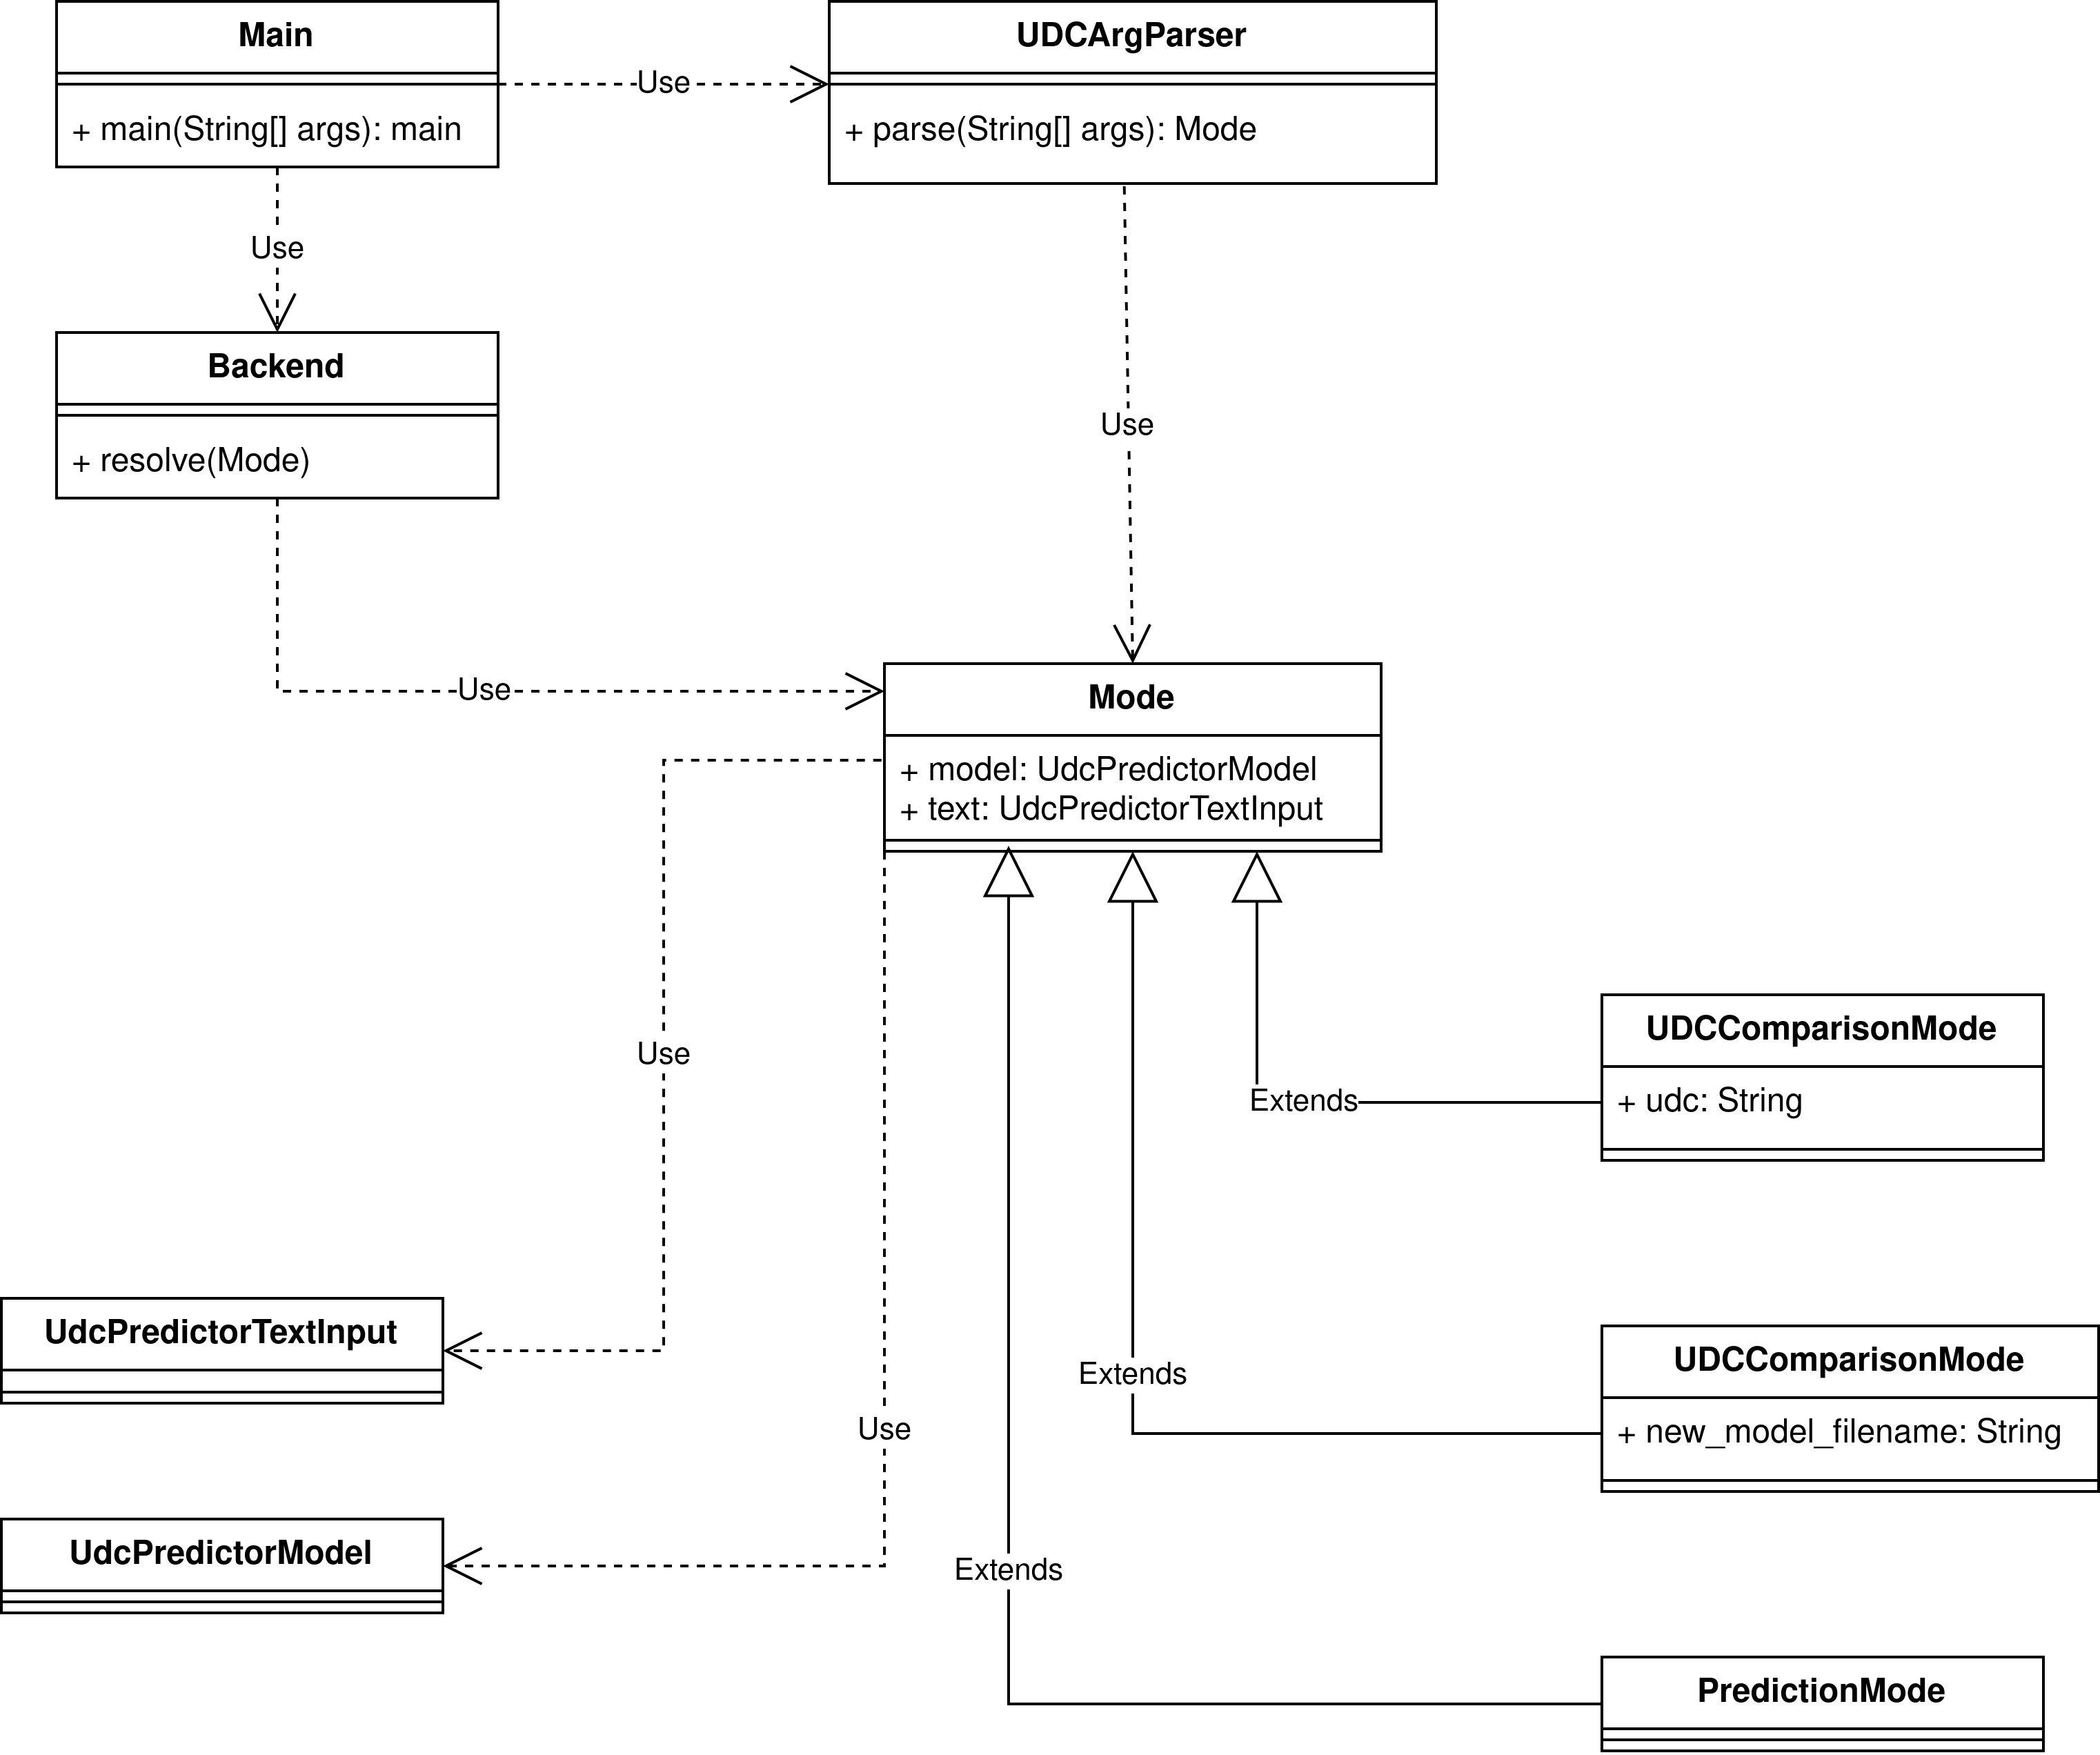
\includegraphics[height=0.6\textwidth]{io_uml5.drawio.png}    
    \caption{Інкапсуляція типів вхідних даних}
    \label{fig:io_uml5}
  \end{sidewaysfigure}

  \newpage

  Через ці зміни, доцільно частково відмінити попередню зміну ---
  тип Mode буде мати імена файлів, а клас Main буде зчитувати та записувати їх.
  Це рішення є покращенням через те що тип
  UDCComparisonMode все ще має ім'я файлу,
  насправді його можна було б замінити на дескріптор файлу,
  алє тоді отримання ресурсу (файлу),
  та його звільнення (закриття) відбувалося б у різних методах та класах ---
  це порушує RAII \cite{wiki_raii}.
  Крім того, на даний момент клас Main не мав явної відповідальності
  (крім посередництва між іншими класами),
  тому ми можемо додати цю роботу до цього модуля.
  Також внутрішня реалізація буде напряму залежати
  від типів UdcPredictorTextInput та UdcPredictorModel.

  Нова версія (рис. \ref{fig:io_uml6}) вирішує вище описані проблеми
  наступним чином:
  \begin{itemize}[labelindent=\dimexpr\parindent*2\relax, leftmargin=*]
    \item внутрішня реалізація тепер має два методи ---
    припущення та тренування,
    вони напряму залежать від типів UdcPredictorModel та \\ UdcPredictorInputText.
    \item тип/клас/модуль UdcCode відподідає за представлення шифрів УДК
    та їх порівняння,
    модуль Main перетворює рядок отриманий від UdcArgParser на цей тип.
    \item усі взаємодії із файлами відбуваются у класі Main.
  \end{itemize}

  \begin{sidewaysfigure}[htbp]
    \centering
    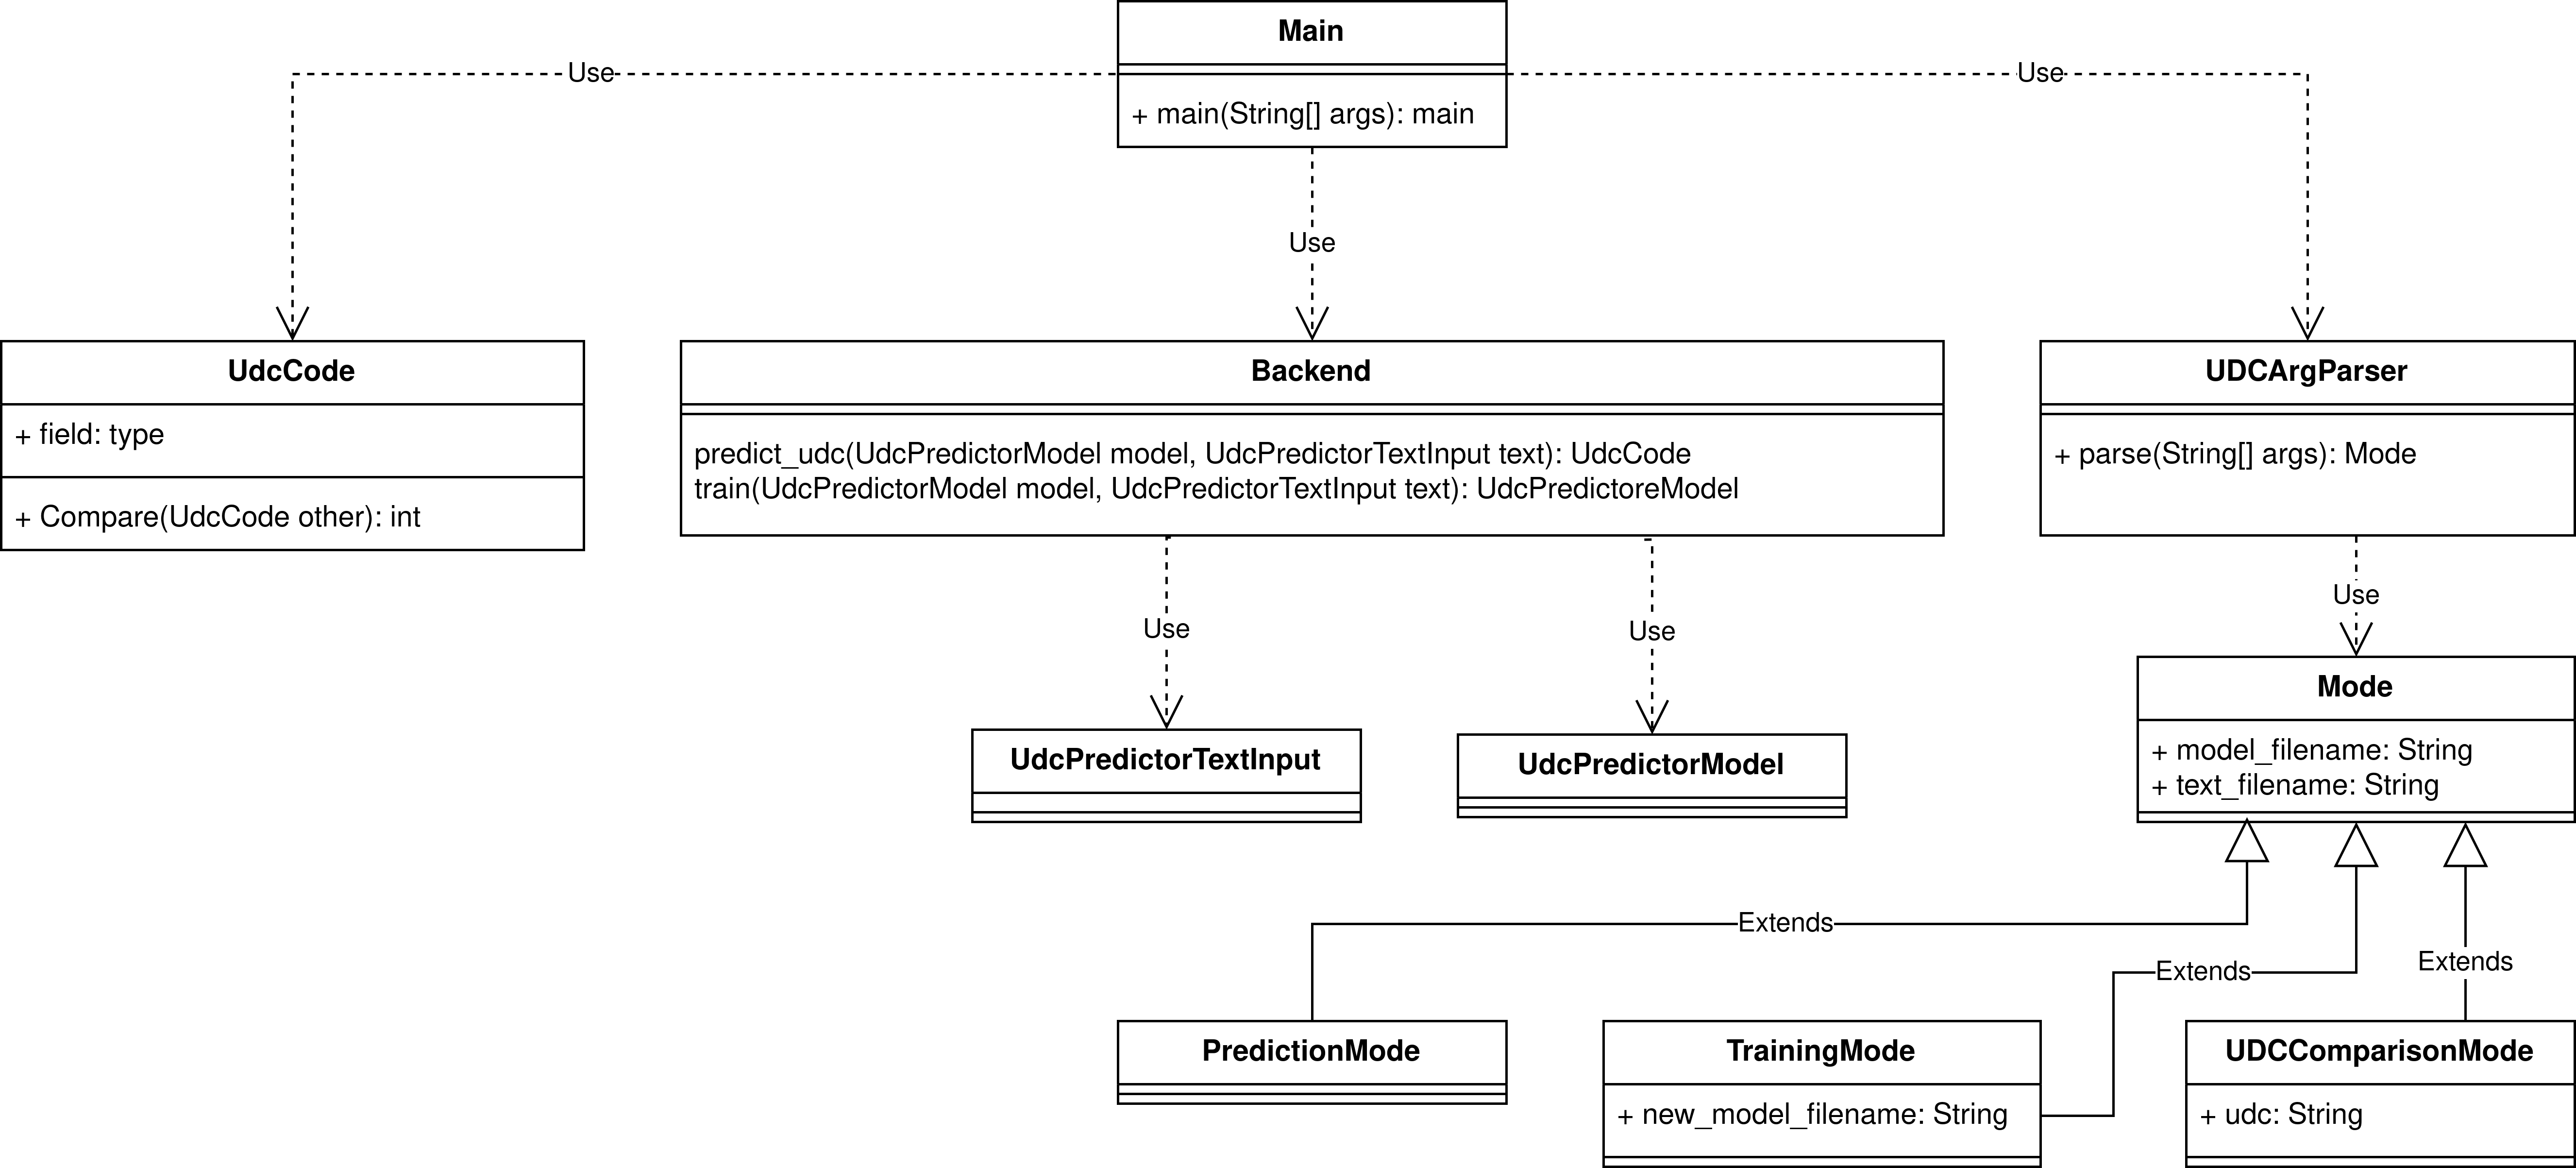
\includegraphics[height=0.45\textwidth]{io_uml6.drawio.png}    
    \caption{Виділення типу для внутрішнього представлення УДК шифрів,
    виділення відповідальностей внутрішньої реалізації,
    перенесення відповідальності за считування файлів}
    \label{fig:io_uml6}
  \end{sidewaysfigure}

  \newpage

  \subsection{Вибір засобів програмування}
  Для реалізації даного ПЗ було обрано мову Python,
  як найпопулярнішу в даному напрямі.
  Крім того,
  через те що ця мова була й залишається однією
  з самих популярних багато років поспіль
  \cite{tiobe_index, pypl, github_octoverse2022, languish}
  (рис. \ref{fig:python_languish}),
  вона має багатий набір різноманітних бібліотек та велику громаду,
  що дозволяє швидко знаходити рішення навіть для складних проблем.

  \begin{figure}[H]
    \centering
    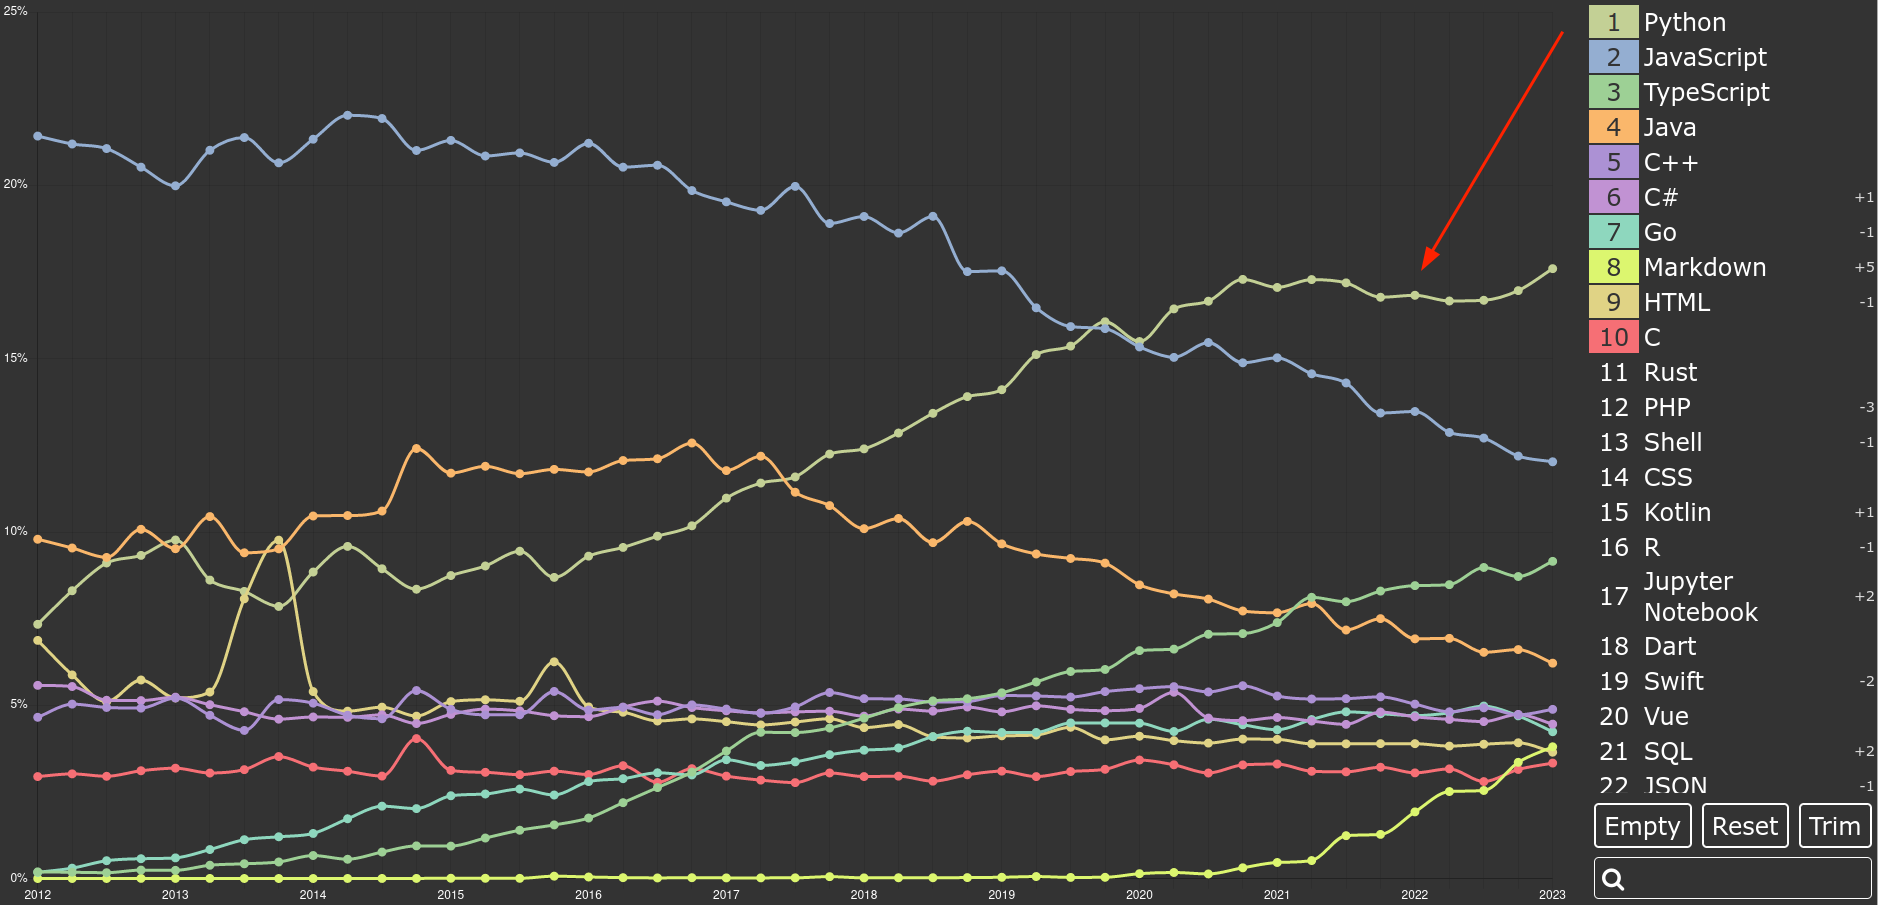
\includegraphics[width=\textwidth]{languish_python.png}    
    \caption{Скриншот графіку популярності мов програмування
    з веб-ресурсу languish}
    \label{fig:python_languish}
  \end{figure}

  Для вирішення задачі отримання ключових слів для заданого тексту
  потрібен такий функціонал:
  \begin{itemize}[labelindent=\dimexpr\parindent*2\relax, leftmargin=*]
    \item токенізація,
    \item видалення стоп слів \cite{wiki_stop_word},
    \item розмічування частин мови \cite{wiki_pos_tagging},
    \item розпізнавання іменованих сутностей \cite{wiki_ner}.
  \end{itemize}

  Альтернативою може бути бібліотека, яка б надавала готовий алгоритм,
  наприклад:
  \begin{itemize}[labelindent=\dimexpr\parindent*2\relax, leftmargin=*]
    \item RAKE (Rapid Automatic Keyword Extraction) \cite{rake_nltk},
    \item YAKE (Yet Another Keyword Extractor) \cite{pypi_yake},
    \item spaCy \cite{spaCy},
    \item NLTK (Natural Language Toolkit) \cite{nltk},
    \item TextBlob \cite{TextBlob},
    \item Gensim \cite{gensim}.
  \end{itemize}

  YAKE потребує тренування на конкретному наборі даних ---
  не підходить для цього випадку з тієї самої причини що й класифікація.

  TextBlob є високорівневою обгорткою над NLTK,
  тому їх доцільно розглядати разом.
  Це бібліотеки загального призначення,
  але їх можна відкинути з наступних причин:
  \begin{itemize}[labelindent=\dimexpr\parindent*2\relax, leftmargin=*]
    \item вони програють spaCy за швидкістю,
    \item spaCy має кращі моделі,
    \item spaCy має більш просунуті функції.
  \end{itemize}

  Хоча spaCy не має готового алгоритму витягування ключових слів,
  його дуже легко реалізувати.

  Алгоритм, який використовує RAKE працює наступним чином ---
  текст розбивається на слова, потім перевіряється частота слів,
  та ступінь їх появи з іншими,
  слова сортуються за обома критеріями з попереднього кроку.

  spaCy не надає готово алгоритму виділення ключових слів,
  але дає можливість розбити текст на слова, розмічати їх як частини мови,
  розпізнати іменовані сутності.

  Алгоритм RAKE суто статистичний і має більшу похибку ---
  він може вважати за ключові слова такі,
  які не є вагомими та навпаки виключати важливі.

  Gensim не має деяких важливих алгоритмів
  для реалізації витягування ключових слів,
  а ті які є в цій бібліотеці були розроблені, в першу чергу,
  для інших цілей і не є оптимальними для нашої задачі.
  З цього виходить що spaCy є найкращим вибором:
  \begin{itemize}[labelindent=\dimexpr\parindent*2\relax, leftmargin=*]
    \item має весь потрібний функціонал;
    \item має моделі;
    \item швидше за інші бібліотеки.
  \end{itemize}

  \subsection{Висновки}
  Були розглянуті різні типи користувачів,
  сценарії використання додатку цими користувачами.
  Завдяки цьому функціонал ПЗ був розподілений в залежності
  від сценаріїв використання.
  Таке розподілення є корисним для розробки архітектури програми та,
  в подальшому, написання реалізації.

  Було розроблено високорівневу архітектуру програми ---
  виділено модулі та типі, які будуть використані при розробці програми.
  Завдяки використаному ітераційному підходу розробки
  архітектури було помічено та виправлено можливі проблеми ще до написання коду.

  Окрема секція приділена вибору засобів програмування.
  Було порівняно сучасні популярні бібліотеки для мови Python
  та обрано найкращий для реалізації задачи.
  Мову Python було обрано як варіант з найбільшою підтримкою бібліотек
  для машинного навчання.

  \section{РОЗРОБКА ПРОГРАМИ}
  \subsection{Розробка інтерфейсу користувача}
  Для простоти виконання буде використано інтерфейс командного рядка (CLI). 
  Для цієї задачі в мові python є спеціалізований модуль argparse.

  З розробленої use-case діаграми можна сказати шо є два режими роботи
  (стільки  ж скільки й акторів).
  Через те що режими тільки два, доцільно використати прапор.
  Основним сценарієм є припущення,
  тому прапор буде використовуватися для тренування "\-\-training".
  
  Модель та текст присутні на вході кожного випадку,
  тому їх можна зробити позиційними аргументами.
  
  Список класів є тільки в одному випадку,
  тому це буде опціональним аргументом,
  який буде прийматися тільки якщо відсутній прапор "\-\-training",
  цей аргумент буде помічатись як "\-\-udc".
  Для припущення результат буде надаватися в stdout у наступному форматі:
  список класів та ступінь їх відповідності, якщо використано "\-\-udc".
  
  Маємо такі сценарії використання:
  \begin{enumerate}[labelindent=\dimexpr\parindent*2\relax, leftmargin=*]
    \item Тренування моделі
      \begin{mycode}[caption={Тренування моделі}, label={code:training_ex}]
        $ udc-classifier \
            model.model \
            scientific-work.txt \
            --training updated-model.model
      \end{mycode}
      \begin{itemize}
        \item udc-classifier --- назва виконуваного файлу
        \item model.model --- назва файлу існуючої моделі
        \item scientific-work.txt --- назва файлу з текстом наукової роботи
        \item updated-model.model --- назва файлу, до якого буде записано нову модель
      \end{itemize}
    
    \item Отримання припущення
      \begin{mycode}[caption={Отримання припущення}, label={code:result_prompt_ex}]
        $ udc-classifier model.model scientific-work.txt
      \end{mycode}
      \begin{mycode}[caption={Припущення (класи, які можуть підійти до наданого тексту)}
                    , label={code:result_ex}]
        539.120 94 084.3
      \end{mycode}
      \begin{itemize}
        \item udc-classifier --- назва виконуваного файлу
        \item model.model --- назва файлу існуючої моделі
        \item scientific-work.txt --- назва файлу з текстом наукової роботи
      \end{itemize}

    \item Отримання припущення та порівняння класів
      \begin{mycode}[caption={Отримання припущення та порівняння класів}, label={code:result_prompt_ex2}]
        $ udc-classifier \
            model.model \
            scientific-work.txt \
            --udc ‘913(574.22)"19"(084.3)’
      \end{mycode}
      \begin{mycode}[caption={Припущення}
                    , label={code:result_ex2}]
        539.120 94 084.3
        0.3
      \end{mycode}
      \begin{itemize}
        \item udc-classifier --- назва виконуваного файлу
        \item model.model --- назва файлу існуючої моделі
        \item scientific-work.txt --- назва файлу з текстом наукової роботи
        \item третій рядок прикладу ---
        класи, які можуть підійти до наданого тексту
        \item другий рядок --- вхідний шифр УДК
        \item четвертий рядок --- ступінь відповідності класів
        (від 0 до 1, де 0 --- відсутні співпадіння, 1 --- повне співпадіння)
      \end{itemize}
  \end{enumerate}

  \subsection{Перетворення ключових слів на класи УДК}
  В наведених у попередніх розділах відкритих каталогах УДК
  кількість ключових слів для кожного з підкласів дуже мала
  (близько 10 на кожен підклас), тому буде згенеровано свій каталог.
  Алгоритм створення наступний:
  \begin{enumerate}[labelindent=\dimexpr\parindent*2\relax, leftmargin=*]
    \item Беремо ключові слова з існуючої роботи (ті які надав автор),
    \item Витягуємо ключові слова з тексту з допомогою обраного алгоритму,
    \item Порівнюємо ключові слова з п.1 та п.2 та додаємо до каталогу ті,
    які входять до обох списків.
  \end{enumerate}

  Точність такого підходу буде напряму залежати від кількості розглянутих робіт
  та кількості отриманих ключових слів.
  Через обмежений час такі каталоги будуть створені не для усіх підкласів,
  та деякі класи будуть мати меншу вибірку.

  Для розуміння формату моделі,
  яка буде у подальшому використовуватися для припущень,
  доцільно деталізувати цей алгоритм.
  Так як модель буде змінюватися незалежно від коду --- це дані,
  які будуть зберігатися окремо від коду --- у файлі.
  Через це потрібно обрати формат серіалізації
  \cite{wiki_serialization,wiki_serialization_comparison}.

  \subsubsection{Вибір формату серіалізації}

  Для порівняння популярних форматів можна звернутися до статті
  «A Comparison Of Serialization Formats»
  \cite{mbedded_ninja_serialization_comparison} на веб-ресурсі mbedded.ninja
  \cite{mbedded_ninja}.

  Розглянемо критерії за якими ця стаття порівнює формати, та оберемо ті,
  які є важливими:

  \begin{itemize}[labelindent=\dimexpr\parindent*2\relax, leftmargin=*]
    \item стислість --- цю характеристику можна вважати однією з складових
      читабельності,
      тому для простоти порівняння вона не буде включена у порівняльну таблицю;
    \item читабельність --- хоча дані,
      які будуть серіалізуватися здебільшого орієнтовані на читання не людиною,
      а комп'ютером,
      іноді можуть виникати ситуації коли буде читабельність є важливою.
      Наприклад --- налагодження;
    \item підтримка мов програмування --- ця характеристика є важливою
      для сумісності \cite{wiki_interop}
      з можливими розширеннями на інших мовах програмування;
    \item структура даних --- ця характеристика має відносно низьку важливість.
      Вона має значення тільки у тих випадках, коли оцінка дуже низька,
      що свідчить про погану гнучкість
      і необхідність незручного перетворення деяких структур даних;
    \item швидкість --- ця характеристика дуже залежна від реалізації
      тому не буде порівнюватися.
      Крім того, в цьому додатку швидкість не є критичною характеристикою,
      відповідно це стосуєтся і складових додатку;
    \item стандартизація --- без цієї характеристики
      підтримка різних мов програмування має мало сенсу.
  \end{itemize}

  Представимо важливу для нас частину даних з наведеного раніше ресурсу
  у вигляді таблиці (\ref{tab:serialization_comparison})
  для простішого вибору формату серіалізації.

  \begin{table}
    \centering
    \rotatebox{90}{
      \begin{minipage}{\textheight}
        \begin{tabular}{|c|c|c|c|c|}
          \hline
          Формат   & Підтримка мов програмування & Читабельність & Структура даних & Стандартизація \\
          CSV      & 9/10                        & 5/10          & 3/10            & 3/10 \\
          JSON     & 9/10                        & 5/10          & 6/10            & 9/10 \\
          Protobuf & 7/10                        & 1/10          & 8/10            & 9/10 \\
          TOML     & 6/10                        & 9/10          & 9/10            & 9/10 \\
          XML      & 9/10                        & 5/10          & 9/10            & 10/10 \\
          YAML     & 6/10                        & 7/10          & 10/10           & 8/10 \\
          \hline
        \end{tabular}
        \caption{Порівняння форматів серіалізації}
        \label{tab:serialization_comparison}
      \end{minipage}
    }
  \end{table}

  Одразу ж доцільно відкинути CSV \cite{wiki_csv}
  за низьку оцінку в структурі даних --- підтримуются тільки таблиці,
  та Protobuf \cite{wiki_protobuf} за дуже низьку оцінку в читабельності.

  Наступним кроком відкидаємо JSON \cite{wiki_json}
  та XML \cite{wiki_xml} через погану читабельність.

  Залишаєтся обрати з TOML \cite{wiki_toml} та YAML \cite{wiki_yaml}.
  Підтримка мов програмування у обох
  варіантів має однакову оцінку тому будемо обирати за іншими характеристиками.
  Найпростіше буде скласти інші оцінки та обрати варінт із більшою сумою,
  за таким порівняння виграє TOML (9+9+9=27) проти YAML (7+10+8=25).
  Можна також обрати той варіант який виграє по більшій кількості показників,
  тут також виграє TOML - два проти одного.

  Можна було б використати складніші способи порівняння,
  наприклад для кожної з обраних характеристик можна додавати множник
  важливості, і порівнювати суму значень з множниками.
  Алє на першому етапі розробки для цього додатку це рішення не є практичним ---
  набагато краще було б отримати відгуки реальних користувачів,
  і вже на його основі можливо змінювати формат серіалізації,
  або додавати підтримку нового.

  Було обрано TOML (акронім "Tom's Obvious, Minimal Language").
  Крім вже оглянутих характеристик,
  можна додати що цей формат має синтаксис дещо схожий на Python,
  це можна вважати плюсом тому що дозволяє розробнику,
  та можливу користувачи витрачати меньше єнергії
  на перехід від коду до серіалізованих даних \cite{Code_complete_5_2}.
  Ця ситуація є схожою на JavaScript та JSON,
  тож якщо цей додаток був би написаний на JavaScript
  то JSON мав би додаткову перевагу.

  Крім того слід додати що вибір популярного
  та добре стандартизованого формату дозволяє мати більшу сумісність
  з іншими форматами завдяки конверторам з одного формату в інший
  \cite{github_json2toml,github_xmltodict,github_x2js}.
  
  \subsubsection{Формат моделі}

  Під час тренування моделі клас УДК буде вважатися таким,
  що відповідає ключовому слову (або навпаки),
  якщо ключове слово підібране програмою наявне у списку ключових слів,
  підібраних автором.
  Ця відповідність між ключовим словом та класом буде додана до моделі.
  Класи УДК в даному випадку будуть надані користувачем для тренування.

  Крім того, в подальшому, для звуження множини рекомендованих класів,
  можна буде додати систему рангування відповідальності між ключовим словом
  та класом.

  По перше, доцільно допускати до тренування лише підмножину ключових слів
  підібраних програмою \cite{wiki_sampling}.
  На даний момент допускаєтся 50 найпопулярніших ключових слів ---
  такий критерій було обрано здебільшого довільно, через обмежений час ---
  за можливості доцільно було б порівняти різні способи вибірки
  \cite{wiki_sampling_methods}
  підмножин ключових слів.

  По друге, можна рангувати \cite{wiki_weight_function}
  кожну пару з класу УДК та ключового слова
  в відповідальності до того як часто зустрічаєтся таке ключове слово
  у текстах із відповідним класом УДК.
  Найпростішим рішенням буде використання кількості
  використань ключового слова у усіх текстах використаних для тренування
  (із таким класом УДК),
  тобто просто сумувати кількість використань у кожному тексті.
  Такий підхід скоріш за все покращить точність, алє він не є ідеальним ---
  різні тексти будуть мати різну довжину,
  тому кількість використань буде пропорційно змінюватись.
  Крім того, частота використання слів може мати різну пропорцію навіть
  у текстах схожих розмірів, тому доцільно було б використовувати відносну
  частоту --- кількість використання слова у тексті,
  поділену на кількість використань усіх ключових слів.
  Можна використовувати й інші формули ---
  частоту відносно усього текста тощо,
  усі вони будуть точніше ніж проста кількість,
  алє щоб підібрати найкращу доцільно проводити порівняння
  на великих наборах даних.

  В цілому усі розглянуті варіанти мають спільні характеристики ---
  пара з ключового слова та класу УДК,
  деякі підходи також додають вагу до кожної пари для обмеження кількості
  рекомендованих класів --- можна обирати N класів із найбільшою вагою,
  або усі класи, вага яких перевишує деякий поріг ---
  який з цих підходів є кращім теж доцільно перевіряти на практиці.

  Таку модель можна зберігати у вигляді таблиці із цих трьох
  (у деяких випдках двох значень).
  Завдяки обраному відносно універсальному формату (де)серіалізації,
  натренована модель може бути використана у інших програмах,
  написаних на різних мовах програмування.

  Для додатку, розроблюваного у даній роботі,
  було вирішено додати для кожного запису вагу,
  а саме --- кількість використань ключового слова
  в усіх текстах із наведеним  класом, які були використані під час тренування. 

  \subsubsection{Алгоритм перетворення ключових слів на класи УДК}
  Ця секція пропонує початковий алгоритм, який може буде покращений,
  або замінений при наявності необхідного часу.

  Першим кроком є витягування ключових слів з тексту ---
  цьому кроку буде приділено окремий розділ цієї роботи.

  Наступним кроком потрібно залишити лише ті ключові слова, які є у списку,
  наданому користувачем.

  Далі для кожного з класів УДК, наданих користувачем,
  додамо до моделі запис для кожного з залишившихся ключових слів із цим класом,
  ключовим словом, та кількістю використань цього слова.
  Якщо запис із таким класом та ключовим словом вже присутній ---
  просто збільшуємо лічильник використань такого ключового слова.

  Цей алгоритм можно представити математичною формулою
    (\ref{eq:keywords_to_classes}).
  \begin{equation}
    \begin{alignedat}{3}
      F := &\{~ (k,~ n(k,&&~ K)) ~|~ k \in K,~ &&K = K_p \cap K_u ~\} \\
      M':= &\{~ (k,~ f)  &&|~ (k, f)          &&~\forall ((k, f') \notin F
           \land   (k, f) \in M) \\
           &             &&                    &&\lor   ((k, f) \in F
           \land   (k, f') \notin M) \\
           &             &&,~ (k,~ f_f + f_m) &&~\forall (k, f_f) \in F \\
           &             &&                    &&\land   (k, f_m) \in M \\
           &\}
    \end{alignedat}
    \label{eq:keywords_to_classes}
  \end{equation}

  Де $F$ --- ключові слова (та кількість їх використань),
      які були підібрані програмою та присутні у списку, який надав користувач.
  $K_p$ --- ключові слова підібрані програмою,

  $K_u$ --- ключові слова надані користувачем,

  $n(k,~ K)$ --- скільки разів $k$ зустрічаєтся в $K$,

  $M$ --- старе значення моделі (такий самий формат я і в $F$),

  $M'$ --- нове значення моделі,

  $f'$ --- будь яке значення f (wildcard).

  \subsubsection{Алгоритм витягування ключових слів}
  У додатку використано функціонал бібліотеки spaCy,
  тому ця секція розглядає алгоритм \cite{wiki_algorithm} на рівні абстракції
  \cite{wiki_abstraction,wiki_abstraction_layer}
  з використанням цієї бібліотеки.
  Огляду реалізації використаного функціоналу буде приділено окрему секцію.

  Для витягування ключових слів використано наступні кроки:
  \begin{enumerate}[labelindent=\dimexpr\parindent*2\relax, leftmargin=*]
    \item Виберемо з тексту іменникові групи ---
      для цього використано функціонал бібліотеки SpaCy.
      Під іменниковою групою маєтся наувазі словосполучення,
      яке описує один об'єкт, наприклад «злий чорний кіт».
    \item Виключемо іменникові групи у яких є стоп-слова \cite{wiki_stop_word}.
    \item Видалимо розділови знаки із залишившихся груп.
    \item Видалимо усі групи, де довжина тексту не перевищує одного символу.
    \item Перетворимо усі літери до нижнього регістру.
    \item Підрахуємо частоту використання кожної з груп.
    \item Відсортуємо групи за частою їх використання в порядку спадання.
    \item Виберемо N найпопулярніших.
  \end{enumerate}

  Математично це може бути записано такою формулою (\ref{eq:keywords}).
  \begin{equation}
    \begin{alignedat}{2}
     keywords := ~&\{~ x \\
                  &|~ n \in N &&~~,  ~ x = lowercase(n \setminus P) \\
                  &           &&~~,  ~ x \cap S = \varnothing \\
                  &           &&\land~ | text(x) | > 1 \\
                  &           &&\land~ rank(x) <= c \\
                  &\}
    \end{alignedat}
    \label{eq:keywords}
  \end{equation}

  Де n --- іменникова група,
  
  N --- множина іменникових груп,
  
  S --- множина стоп слів,
  
  w --- слово в іменниковій групі,
  
  P --- множина знаків пунктуації,
  
  rank --- функція,
      яка повертає позицію елемента у множині за популярністю
      у порядку спадання,
  
  c --- кількість ключових слів, які потрібно обрати.

  \subsubsection{Огляд алгоритму spaCy noun\_chunks}
  Бібліотека spaCy має натреновані моделі \cite{spacy_models,spacy_pipelines},
  які зазвичай складаются з:
  \begin{itemize}[labelindent=\dimexpr\parindent*2\relax, leftmargin=*]
    \item токенізатору \cite{wiki_tokenizer,spacy_tokenizer} ---
      цей процесс відповідає за виділення окремих слів з тексту,
    \item розмічувального алгоритму \cite{spacy_tagger} ---
      цей алгоритм розмічує слова за частинами мови \cite{wiki_pos_tagging},
    \item лемаматизатору \cite{spacy_lemmatizer} ---
      цей компонент відповідає за лемматизацію \cite{wiki_lemmatization} ---
      процесс приведення слова до лемми \cite{wiki_lemma} ---
      нормальної форми слова,
    \item парсеру \cite{spacy_dependency_parser} --- ця частина алгоритму розпізнає синтаксичні
    залежності між словами.
    \item розпізнавачу іменованих сутностей \cite{wiki_ner, spacy_er}
  \end{itemize}

  Цю послідовність можно представити графічно (рис. \ref{fig:spacy_pipeline}).
  Токенайзер завжди виконуєтся першим
  тому що усі послідуючі крокі працюють з окремими словами.
  Інші компоненти зазвичай ніяк не залежать один від одного,
  тому порядок їх виконання не є важливим. Втім,
  бібліотека підтримує і сторонні моделі, які можуть мати додаткові кроки,
  і вже вони можуть мати фіксований порядок виконання відносно один одного
  та стандартних кроків.

  \begin{figure}[H]
    \centering
    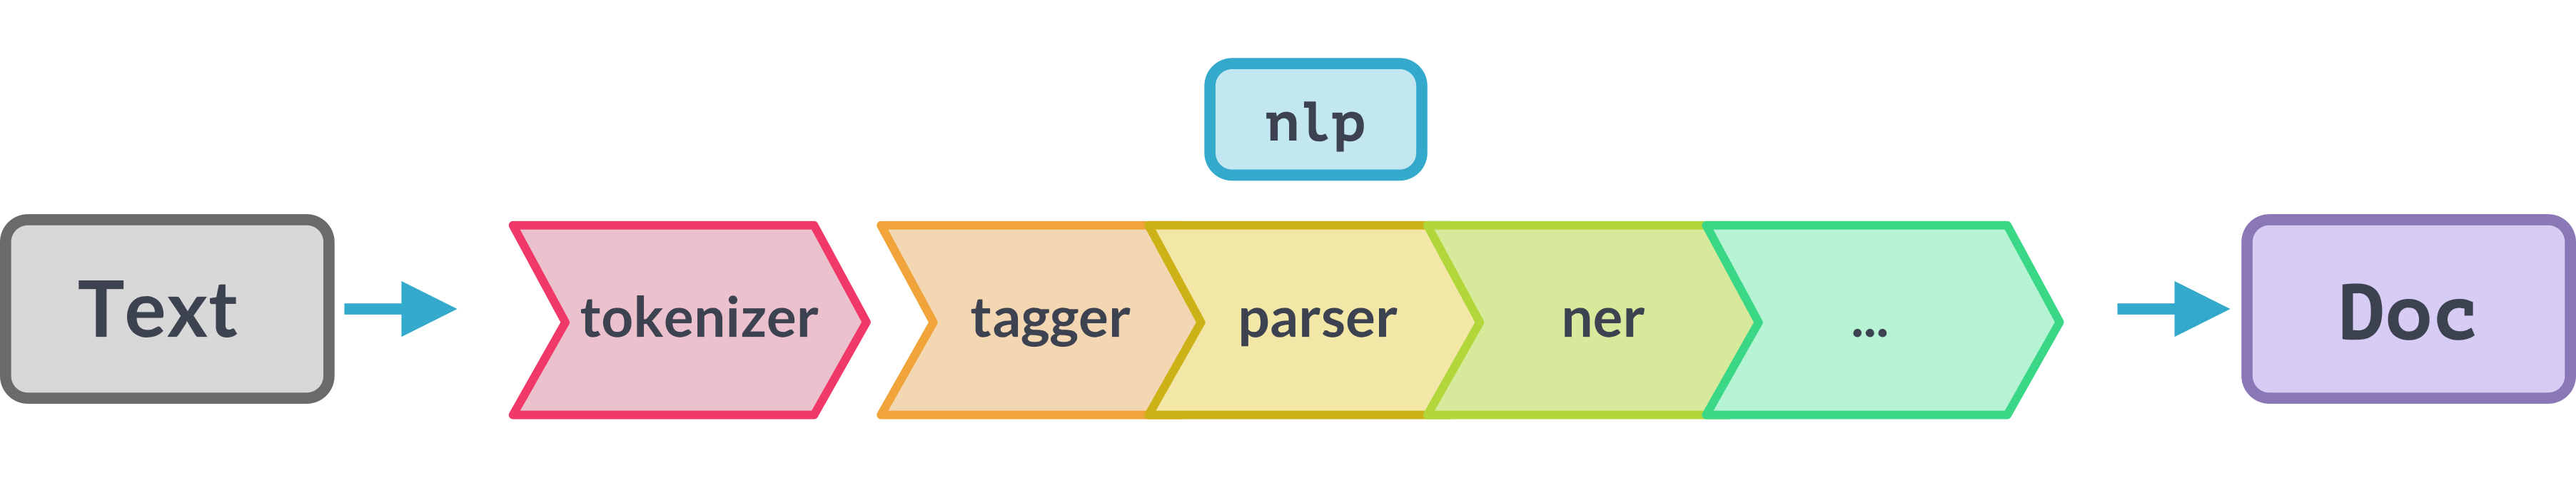
\includegraphics[width=\textwidth]{spacy_pipeline.png}    
    \caption{Послідовність розбірки тексту моделями бібліотеки spaCy}
    \label{fig:spacy_pipeline}
  \end{figure}

  Після обробки стандартним алгоритмом над документом можна проводити додаткові
  трансформації, однією з них є функція noun\_chunks
  \cite{spacy_noun_chunks} ---
  вона повертає усі іменникові групи \cite{wiki_noun_phrase} в тексті.

  Функція noun\_chunks працює наступним чином \cite{wiki_noun_chunks_impl}:

  \begin{enumerate}[labelindent=\dimexpr\parindent*2\relax, leftmargin=*]
    \item Залишаємо лише ті слова, які помічені як іменники,
      займенники або власні ім'я --- цю інформацію надає розмічувач частин мови.
    \item Обходимо залишені слова:
    \begin{enumerate}
      \item Якщо слово вже було використано в групі -- пропускаємо.
      \item Якщо слово помічено як залежне з однією з наступних залежностей -- додаємо це, та наступне слово як іменникову групу.
        Ці залежності проставляє парсер \cite{spacy_label_scheme}:
        \begin{enumerate}
          \item "oprd" (Object Predicate) \cite{wiki_predicate_grammar} ---
            присудок,
          \item "nsubj" (Nominal Subject) \cite{nsubj_dep} --- називний підмет,
          \item "dobj" (Direct Object) \cite{wiki_dobj} --- прямий додаток,
          \item "nsubjpass" (Passive Nominal Subject) \cite{nsubj_pass_dep} ---
            називний підмет в орудному відмінку,
          \item "pcomp" (Prepositional Complement)
            \cite{wiki_prepositional_phrases} --- прийменникове доповнення,
          \item "pobj" (Prepositional Object) --- прийменниковий додаток,
          \item "dative" (Dative) \cite{wiki_dative} --- давальний відмінок,
          \item "appos" (Appositional Modifier) \cite{appos_dep} --- прикладка,
          \item "attr" (Attribute) \cite{wiki_grammatical_modifier} ---
            означення,
          \item "ROOT" \cite{root_dep} --- корінь речення,
            зазвичай головний присудок або дієслово речення.
        \end{enumerate}
     \item Якщо слово помічено залежністю «conj» (сполучення)
       \cite{wiki_conjunction, conj_dep}
       (наприклад «та», «або»),
       додаємо це, та інші слова які помічені як залежні в цій групі.
    \end{enumerate}
  \end{enumerate}

  \subsection{Висновки}
  Було розроблено користувацький інтерфейс,
  розроблено алгоритм перетворення ключових слів на класи УДК.
  Також було порівняно різні методи серіалізації даних,
  та було обраний найкращий для цільової проблеми.
  Розроблено алгоритм витягування ключових слів з тексту за
  домопомогою бібліотеки spaCy. Крім того, розглянуто алгоритм,
  за яким ця бібліотека разбирає текст що дозволяє нам витягувати
  з нього ключові слова та виконувати над ним інші трансформації.

  \section{ТЕСТУВАННЯ КОРИСТУВАЦЬКОГО ІНТЕРФЕЙСУ}
  Функціонал розробленого додатку неможливо оцінити бінарно як працює або
  не працює, або навіть дискретно. Хоча й дійсно додаток може не працювати,
  алє процювати ідеально він не може тому що не існує стандарту за яким
  би можна було перевірити коректність роботи. Натомість можливо порівняти
  результати які надає розроблена програма із тими, які були підібрані авторами
  робіт, або бібліотекарями. Натомість, таке порівняння не є можливим у
  рамках цієї роботи тому що для того щоб зробити вагомі висновкі необхідний
  достатньо великий набір даних --- при маленький вибірці програмі може просто
  «пощастити» і вона порекомендує дуже точно, також може бути і навпаки,
  алє з великим набором даних такі похибки не будуть заважати середньому
  результату.

  Хоча протестувати саме цільовий функціонал і неможливо,
  можна протестувати користувацький інтерфейс.
  По-перше, доцільно описати можливі вхідні дані.
  При нормальному використанні програма очікує два обов'язкових аргументи ---
  model\_filename (путь до файлу моделі) та
  text\_filename (путь до файлу із текстом для класифікації).

  Крім того програма може приймати три опціональних параметри:
  \begin{itemize}[labelindent=\dimexpr\parindent*2\relax, leftmargin=*]
    \item training --- цей параметр означає що програма має відпрацювати
      у режимі тренування,
      за цим параметром надаєтся путь файлу для збереження нової моделі.
    \item udc --- цей параметр приймає класи,
      які можуть бути використані для порівняння із класами
      підібраними програмою або для тренування моделі,
      в залежності від обраного режиму роботи.
    \item keywords --- за цим параметром передаєтся набір ключових слів
      для використання під час тренування моделі.
  \end{itemize}

  \newpage
  Слід додати що для кожного з режимів необхідний конкретний
  набір опціональних аргументів, а саме:
  \begin{itemize}[labelindent=\dimexpr\parindent*2\relax, leftmargin=*]
    \item для тренування --- training, udc та keywords,
    \item для припущення та порівняння --- udc,
    \item для припущення не потрібен жоден з опціональних аргументів.
  \end{itemize}

  Також є додаткові аргументи '-h' та '-{}-help' ---
  обидва виводять на екран інформацію про програму.
  Якщо програму запущено із некоректними аргументами -- виводится рядок,
  в якому написані можливі аргументи, та рядок із помилкою.

  Для тестування пропонуєтся розробити таблицю, де рядками будуть тести,
  а стовпцями будуть аргументи, значення кліток ---
  присутність або відсутність зазначеного аргумента у зазначеному тесті.
  Також слід додати один стовпець для неочікуваного аргументу.
  Слід зазначити що усі випадки де аргументи присутній,
  будуть використовувати коректне значення для цього аргументу.
  Такий спосіб тестування можна вважати таким,
  що належить до методу сірої скриньки ---
  усі ці тести тестують тільки один з модулів ---
  ця інформація доступна лише розробнику, але ми не виключаємо комбінації
  які належать до одних й тих самих класів еквівалентності.

  Насправді через кількість можливіх комбінацій ($2^6 = 64$),
  доцільно виключити деякі тести, а навіть групи.

  По перше з документації бібліотеки argparse нам відомо що при вказаному
  аргументі -h або -{}-help завжди буде виведено інформаційне повідомлення,
  незалежно від усіх інших параметрів, тому доцільно залишити
  один тест де усі парамети крім цього відсутні,
  а в усіх інших тестах не вказувати цей параметр,
  таким чином ми залишаємо лише ($2^5 + 1= 33$) тестів, що майже вдвічи менше.

  Також, нам відомо що при виявлені неочікуваного параметру
  буде показане повідомлення про помилку незалежно від інших аргументів.
  Тому доцільно залишити один тест із коректними неопціональними параметрами
  та вказаним неочікуваним аргументом,
  в усіх інших випадках неочікуваний параметр вказувати не будемо.
  Таким чином ми залишаємо тільки ($2^4+2=18$) тестів,
  це знову майже вдвічи меньше.

  До того ж, ми знаємо що відсутність будь
  якого з обов'язкових параметрів призведе до помилки,
  тому немає сенсу тестувати випадки де один з них відсутній,
  а інший --- ні.
  Загалом, достатньо залишити лише один тест, де
  відсутні ці та будь які інші параметри,
  а в усіх інших вказувати обов'язкові параметри.
  Завдяки цьому ми знову зменшуємо кількість тестів --- до ($2^3+3=11$).
  Таким чином ми виділили велику групу тестів з однаковими результатами
  та замінили їх на лише 3. Крім того, пропущені тести насправді перевіряли
  б бібліотечний код, що не має сенсу тому що він протестований розробниками.
  Решта тестів перевіряє вже функціонал розроблений спеціально для додатку.

  \vspace{\baselineskip}
  \noindent
  \begin{tabular}{|c|c|c|c|c|}
    \hline
    \# & -{}-training & -{}-udc & -{}-keywords & очікування \\
    \hline
    1  & \multicolumn{3}{l|}{тільки -h} & \\
    2  & \multicolumn{3}{l|}{text\_filename, model\_filename та неочікуваний параметр} & \\
    3  & \multicolumn{3}{l|}{text\_filename та model\_filename відсутні} & \\
    \hline
    4  & & & & \\
    5  & & & & \\
    6  & & & & \\
    7  & & & & \\
    8  & & & & \\
    9  & & & & \\
    10 & & & & \\
    11 & & & & \\
    \hline
  \end{tabular}

  \vspace{\baselineskip}
  TODO: maybe add tests for when file is unreadable for whatever reason


  \subsection{Висновки}

  \section{Поширенння додатку}
  Python це здебільшого інтерпретована мова програмування.
  Насправді некоретно казати що саме мова є інтерпретованою або компільованою,
  бо мова лише описує синтаксис та семантику,
  а код може бути і інтерпретованим і компільованим (напр. Dart \cite{dart_lang}),
  алє саме в мові Python офіційний інструмент для запуску програм ---
  інтерпретатор.
  
  Розроблюваний додаток орієнтований не тільки на просунутих користувачів,
  тому доцільно загорнути додаток в автономний пакет,
  щоб звільнити користувачів від встановлення інтерпретатора та бібліотек.

  Для вирішення цієї задачі можна розглянути декілька підходів:
  \begin{itemize}[labelindent=\dimexpr\parindent*2\relax, leftmargin=*]
    \item PyInstaller \cite{pyinstaller} ---
      один з головних претендентів на вирішення задачі.
      На перший погляд,
      ця python бібліотека повністю підходить під вказані вимоги ---
      вона збирає усі скрипти, усі модулі,
      усі бібліотеки та інтерпретатор в один комплект,
      який може бути запущеним кінцевим користувачем без додаткових дій.
      Втім, є деякі недоліки:
      \begin{itemize}
        \item це рішення не є кросплатформенним, тобто «зібрати» виконуваний файл для цільової платформи можна тільки на цій платформі
        \item деякі платформи зовсім не протестовані
      \end{itemize}
      Хоча це рішення є дуже гарним, доцільно розглянути й інші,
      перед тим як робити кінцевий вибір.
    
    \item Nuitka \cite{nuitka} --- python компілятор,
      так само не є кросплатформеним.
      Крім того, це рішення менш популярне ніж PyInstaller,
      та вимагає більшої кількості залежностей.
      Алє, це рішення може бути корисним, якщо додаток,
      зібраний з допомогою PyInstaller буде виконуватись дуже повільно.

    \item py2exe \cite{py2exe} --- цей інструмент орієнтований лише на одну
      операційну систему --- Windows,
      з цієї причини він є гіршим за інші запроновані рішення.
    
    \item Cython \cite{cython} --- самий популярний python компілятор.
    Хоча він також не має прямої можливості компілювати на інші платформи,
    він дозволяє компілювати в код на мові C,
    який у свою чергу можна компілювати на різні цільові платформи з однієї.
    Незважаючи на ці переваги, такий підхід не виграє по зручності PyInstaller,
    алє стоїть на приблизно тому самому рівні, завдяки перевагам над Nuitka.
    
    \item Frozen binaries \cite{github_cpython_freeze} ---
      функціонально те саме що й PyInstaller.
    
    \item Docker \cite{docker} ---
      ця система контейнеризації хоча й сама зручна та стандартизована
      з представлених, вимогає встановлення додаткового ПЗ ---
      через це, це решіння не має сенсу,
      бо ми намагаємося уникнути встановлення додаткового ПЗ
      та спростити встановлення розроблюваного додатку.
    
    \item Cloud-based deployment \cite{wiki_cloud_computing} ---
      найкраща сумістність з різними платформами,
      алє вимагає додаткових ресурсів, та постійного підключення до інтернету.
  \end{itemize}

  Для більш наглядного порівняння можна представити ці дані
  у вигляді такої таблиці:

  \begin{table}
    \centering
    \rotatebox{90}{
      \begin{minipage}{\textheight}
        \begin{tabular}{|c|c|c|c|c|c|c|}
          \hline
          Назва & Кросплатформеність & Тип & Windows & Linux & macOS & FreeBSD/NetBSD \\
          \hline
          PyInstaller & ні & Пакетувальник & 7/8/10/11 & + & >10.15 & +** \\
          Nuitka & ні & Компілятор & + & + & + & + \\
          py2exe & ні & Пакетувальник & + & - & - & - \\
          Cython & так* & Компілятор  & + & + & + & + \\
          Frozen binaries & ні & Пакетувальник  & + & + & + & + \\
          Docker & так & Kонтейнер  & + & + & + & + \\
          Cloud-based deployment & так & веб  & + & + & + & + \\
          \hline
        \end{tabular}

        \vspace{10pt}

        * - можна компілювати не у нативний код, а в код на мові С,
        а вже цей код можна крос-компілювати.

        ** - Неофіційна підтримка

        Nuitka потребує окремого встановлення компілятора gcc
      \end{minipage}
    }
  \end{table}

  \newpage
  З цієї таблиці можна побачити що усі варіанти мають
  підтримку усіх сучасних версій ОС Windows.
  Якщо відкинути py2exe,
  то будь який з варіантів підтримує усі сучасні/популярні ОС.
  Через це залишается обирати з варіантів,
  які дозволяють збирати виконувані файли з під однієї платформи на усі інші.
  Docker вже було виключено через
  те що він замінює одну залежніст від додаткового ПЗ на інше.
  Розгортання веб ресурсу також виключено через додаткові витрати.
  Залишаєтся лише Cython, який підтримує компіляцію на
  будь які цілові платформи з під однієї робочої.

  На практиці виявилося що крос-компіляція з Cython хоча й можлива,
  не є зручною. Головною причиною є погана сумісність компіляторів ---
  python на windows компілюєтся із допомогою компілятора MSVC,
  а крос-компіляція з linux на windows проводится із допомогою mingw.
  Цю проблему можна вирішити перекомпілювавши python із іншим компілятором,
  алє набагато легше буде використовувати цільові ОС для створення
  виконуваних файлів. Для цього доцільно використати PyInstaller.

  Для створення виконуваного файлу потрібно виконати такі кроки:
  \begin{enumerate}[labelindent=\dimexpr\parindent*2\relax, leftmargin=*]
    \item Перейти на цільову платформу.
    \item Встановити python --- для перевірки було використано версію 3.10,
      але скоріш за все підійдуть й інші.
    \item Встановити необхідні залежності:
      \begin{mycode}[caption={Встановлення залежностей}, label={code:install_deps}]
        > pip install spacy
        > python -m spacy download en_core_web_lg
        > pip install pyinstaller
      \end{mycode}
    \item Зібрати виконуваний файл за допомогою PyInstaller:
    \begin{mycode}[caption={Збірка виконуваного файлу}, label={code:install_deps}]
      > pyinstaller ^
          src\main.py ^
          -F ^
          --dist build ^
          --collect-all en_core_web_lg
    \end{mycode}
    Цей приклад використовувася на ОС Windows,
    але він буде працювати і на інших платформах. Єдина суттева зміна ---
    символ продовження строки (\string^), для віндовс це '\string^',
    для unix - '\string\'.
  \end{enumerate}

  В цілому, цей підхід вирішує проблему додаткових залежностей ---
  на виході маємо лише один виконуваний файл. Але можливі деякі покращення:
  \begin{itemize}[labelindent=\dimexpr\parindent*2\relax, leftmargin=*]
    \item Зараз мовна модель запаковуєтся в виконуваний файл.
      Для більшої універсальності можна зробити так,
      щоб модель знаходилась в окремій папці поряд із виконуваним файлом ---
      таким чином користувач за бажанням міг би замінити модель на іншу.
    \item Можна створити docker-контейнери з необхідними платформами
    \cite{docker_windows,docker_windows_base, docker_osx}
      та використовувати їх для збірки виконуваних файлів на
      різні цільові платформи з під однієї платформи розробки.
  \end{itemize}

  \subsection{Висновки}

  Через те що додаток орієнтований на простих користувачів,
  важливо зробити поширення,
  встановлення та використання програми якомога простішим
  для кінцевого користувача. Це є реальною проблемою для цього додатку
  через те що обрані засоби програмування, а саме мова програмування Python,
  роблять поширення складнішим ніж в можливих альтернативах.
  Стається це через те що офіційний спосіб використання цієї мови
  очікує що кінцевий користувач має на своєму пристрої інтерпретатор,
  а розробник у свою чергу поширює вихідний код програми.
  Така парадигма не є зручною бо користувачу потрібно
  окремо встановлювати конкретну версію інтерпретатора,
  а розробнику доцільно якомога швидше оновлювати програму
  для підтримки останніх версій інтерпретатора. Крім того,
  доцільно й підтримувати попередні версії щоб старі користувачі
  могли не оновлювати інтерпретатор кожного разу.
  Тож вцілому це ускладнює і розробку і використання (а саме встановлення)
  додатку.

  Розроблюваний додаток не є першим випадком такої проблеми,
  тому за історію мови Python було розроблено немало способів для вирішення
  цієї проблеми. Ці специфічні для мови Python способи,
  та деякі інші рішення було розглянуто та порівнянно щоб обрати найкращий.
  Перший обраний варіант виявився складнішим у використанні ніж очикувалося,
  тому кінцевий вибір було змінено.

  В підсумку, підібране рішення дозволяє достатньо зручно поширювати
  додаток на різні платформи. Крім того,
  наведено можливі покращення для автоматизації частини роботи для поширення ПЗ.

  \unnumberedSection{ЗАГАЛЬНІ ВИСНОВКИ ТА РЕКОМЕНДАЦІЇ}
  В процесі написання роботи було розроблено додаток,
  який може рекомендувати класи УДК для наданих текстів після тренування.
  Такий додаток може бути корисним для часткової автоматизації
  класифікації великих бібліотек ---
  користувачу достатньо класифікувати тільки частину наукових робіт,
  а для решти можна використовувати рекомендації програми.

  Важливо також зазначити що під час розробки для економії часу було вирішено
  спростити функціонал порівняння шифрів УДК до порівняння списків класів УДК.
  Через це усі використання шифрів УДК було замінено звичайними
  списками класів УДК, а через те що класи УДК представлення простими рядками
  це списки рядків.
  Завдяки цьому рішенню програма стає більш загальною і дозволяє робити
  припущення не тільки у вигляді класів УДК, а й у вигляді класів
  будь яких систем класифікації за умови використання моделі,
  натренованій на відповідних даних.

  Велика частина очевидних покращень складаєтся з порівняння альтернативних
  підходів до використаних рішень --- через обмежений час,
  частина рішень була зроблена без достатнього обгрунтування та/або
  достатнього порівняння альтернатив. Крім того,
  для порівняння частини альтернатив необхіден великий набір данних,
  здобуття якого не є практичним або навіть можливим в межах цієї роботи.

  Інший путь покращень --- користувацький інтерфейс.
  Розроблений функціонал можна вважати перевіркою доцільності такого додатку.
  Алє для комфортного користування додатком можна зробити багато покращень.
  Можна зробити додаток більш модульним --- на даний момент усе,
  крім моделі підбору класів УДК на основі ключових слів,
  запаковане в виконуваному файлі.
  Алє використані засоби програмування дозволяють додати більше можливостей
  для конфігурації, наприклад можна дозволити використовувати різні мовні моделі
  --- це дозволить по-перше за бажаням використовувати простіші язикові моделі,
  які займають менше місця. Крім того,
  це дозволить використовувати додаток із текстами на інших мовах,
  таким чином цей додаток перетворюєтся на фреймворк.
  Також, на основі розробленого інтерфейсу користувацького рядка
  можна розробити графічний інтерфейс ---
  більшості користувачів буде набагато зручніше використовувати додаток
  саме таким чином.

  З точки зору розробки головним покращенням була б автоматизація
  поширення додатку, а саме його пакування у виконуваний файл.
  Це можна вирішити із допомогою контейнеризації цільових платформ
  та використання їх із додатками безпереревної інтеграції.

  Також можна додати рекомендацію яка включає полегшення і розробки,
  і використання --- розгортання додатку у вигляді веб-ресурсу.
  Це не було зроблено у межах роботи через відсутність фінансування.

  Крім того, було б доцільно додати більше стандартів у вигляді вимог
  до написання коду, бажано з автоматизованими перевірками, 
  це б суттево покращило якість вихідного коду,
  що в свою чергу б полегшило подальшу розробку та підтримку додатку.

  Вцілому, розроблений додаток можна вважати гарною
  основою для подальшого розвитку --- завдяки добре розподіленій архітектурі,
  будь-яка частина може бути дуже просто замінена,
  що у свою чергу дозволяє продовжувати ітераційні покращення.

  \phantomsection
  \printbibliography[heading=bibintoc, title=СПИСОК ВИКОРИСТАНОЇ ЛІТЕРАТУРИ]

  \unnumberedSection{ДОДАТКИ}
  \centerline{"../src/udc\_predictor\_text\_input.py"}
\verbatiminput{../src/udc_predictor_text_input.py}
\centerline{"../src/udc\_predictor\_model.py"}
\verbatiminput{../src/udc_predictor_model.py}
\centerline{"../src/mode.py"}
\verbatiminput{../src/mode.py}
\centerline{"../src/udc\_predictor.py"}
\verbatiminput{../src/udc_predictor.py}
\centerline{"../src/udc\_code.py"}
\verbatiminput{../src/udc_code.py}
\centerline{"../src/main.py"}
\verbatiminput{../src/main.py}
\centerline{"../src/parse\_args.py"}
\verbatiminput{../src/parse_args.py}


\end{document}
